\documentclass{article}
\usepackage[polish]{babel}
\usepackage{minted}
\usepackage[letterpaper,top=2cm,bottom=2cm,left=3cm,right=3cm,marginparwidth=1.75cm]{geometry}
\usepackage{amsmath}
\usepackage{graphicx}
\usepackage[colorlinks=true, allcolors=blue]{hyperref}
\usepackage[T1]{fontenc}
\usepackage[table,xcdraw]{xcolor}
\usepackage{float}
\usepackage[figurename=Wykres]{caption}
\usepackage{amsmath}

\title{MOwNiT - Rozwiązywanie równań i układów równań nieliniowych}

\author{Jakub Frączek}

\begin{document}

\maketitle

\section{Wstęp}

Zadanie polegało na wyzaczneniu pierwiastków równania \(f(x) = 0\) na zadanym przedziale [a, b]. W zadaniu należało wykorzystać metodę Newtona i metodę Siecznych, a punkty wybrać co 0.1 na przedziale [a, b]. Dla metody siecznych jeden z końców przedziału miał być ustalony tak jak dla metody Newtona, a drugi jako początek albo koniec przedziału [a, b]. Następnie porównać działania tych metod stosując dwa rózne kryteria stopu.

\section{Funkcja dla której przeprowadzone zostało doświadczenie}

\[f(x) = x^2 - n * sin(x)^m\]

\noindent
gdzie:
\[n = 10, \ m = 15, \ x \in [-1.8, 0.2]\]

\noindent
zatem:

\[f(x) = x^2 - 10 * sin(x)^{15}, \ x \in [-1.8, 0.2]\]

\bigbreak

\noindent
Zatem wykres zadanej funkcji wygląda następująco:

\begin{figure}[H]
  \centering
  \begin{minipage}[b]{0.5\textwidth}
    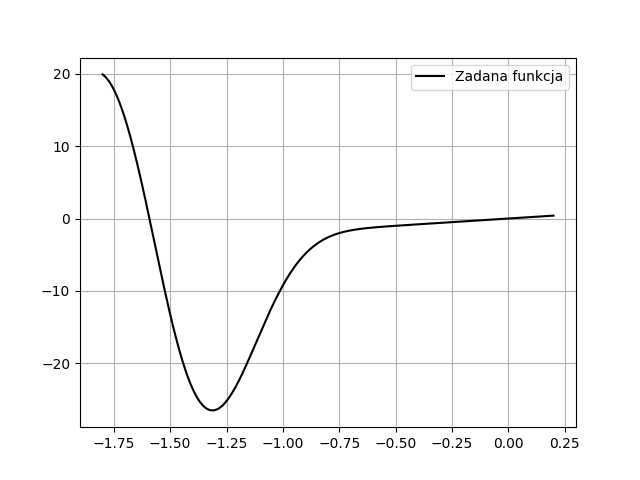
\includegraphics[width=\textwidth]{zadana_funkcja.png}
  \end{minipage}
\end{figure}

\section{Dane techniczne}

\subsection{Hardware}

Laptop z procesorem Intel Core i5-9300H 2.4GHz oraz 32 GB pamięci RAM.

\subsection{Software}

Wykorzystany został system Windows 11 x64 oraz język Python w wersji 3.11.8 wraz z bibliotekami:
\begin{itemize}
\item math
\item enum
\item matplotlib
\item numpy
\end{itemize}

\section{Kryteria stopu}

Kryteria stopu służą do zatrzymania wykonywania programu, gdy przyblizenie miejsca zerowego uznajemy za "dość dobre".

\subsection{Wartość bezwzględna różnicy dwóch ostatnich przybliżeń pierwiastka}

Jednym z kryteriów była wartość bezwzględna rówżnicy dwóch ostatnich przybliżeń pierwiastka równania f(x) = 0.

\[|x^{(i + 1)} - x^{(i)}| < \rho\]

\subsection{Wartość bezwzględna wartości funkcji}

Kolejnym kryterium była wartość bezwzględna wartości funkcji f, w punkcie przybliżającym położenie pierwiastka.

\[|f(x)^{(i)}| < \rho\]

\section{Metoda Newtona}

Do zaimplementowania metody Newtona wykorzystałem wzór:

\[f(\alpha) = 0 = f(x_{i - 1} + h) = f(x_{i - 1}) + h \cdot f'(x_{i - 1}) + ... \ (pomijamy)\]

\noindent
gdzie:

\[\alpha \  - \  prosty \ pierwiastek, \ x \ - \ przblienie \ \alpha, \ h = -\frac{f(x_{x - 1})}{f'(x_{i - 1})}\]

\noindent
zatem otrzymujemy wzór iteracyjny:

\[x_i =x_{i - 1} - \frac{f(x_{i - 1})}{f'(x_{i - 1})}\] 

\section{Metoda siecznych}

Do zaimplementowania metody siecznych wykorzystałem wzór:

\[x_{i + 2} = x_{i + 1} - \frac{x_{i + 1} - x_i}{f_{i + 1} - f_i} \cdot f_{i + 1}\]

\bigbreak

\noindent
Przy czym, startujemy z \(x_0, \ x_1\) i nie badamy \(f_0 \cdot f_1\)

\newpage

\section{Wyniki}

Analizę przeprowadziałem dla wartości \(\rho \in [10^{-1},\ 10^{-20}]\), wartości x zaczynając od początku dziedziny, robiąc krok co \(0.1\) i kończąc lewym krańcu przedziału. Za maksymalną liczbę iteracji wybrałem liczbę 1000. Dodatkowo analiza została przeprowadzona dla dwóch różnych kryteriów stopu.

\subsection{Wyniki dla metody Newtona}

 Wyniki zostały podzielone ze względu na kryterium stopu oraz wartości parametru \(\rho\). Poza tym, w każdym przypadku \(x \in [-1.8, \ 0.2]\).

\subsubsection{Kryterium wartości bezwzględnej wartości funkcji, \(\rho \in [10^{-1}, \ 10^{-10}]\)}

Jak widać na poniższych wykresach, dla \(x = 0\) nie udało się obliczyć wartości pierwiastka, z kolei w innych punktach była ona dośc bliska prawdziwej wartości, a precyzja zwiększała się wraz z zwiększeniem dokładnośći (zmniejszeniem wartości pamametru \(\rho\)). Jak widać zwiększanie dokładności oraz oddalenie od położenia pierwiastka prowadzi do zwiększenia liczby iteracji, ale nie do spadku dokładności.

\begin{figure}[H]
  \centering
  \begin{minipage}[b]{\textwidth}
    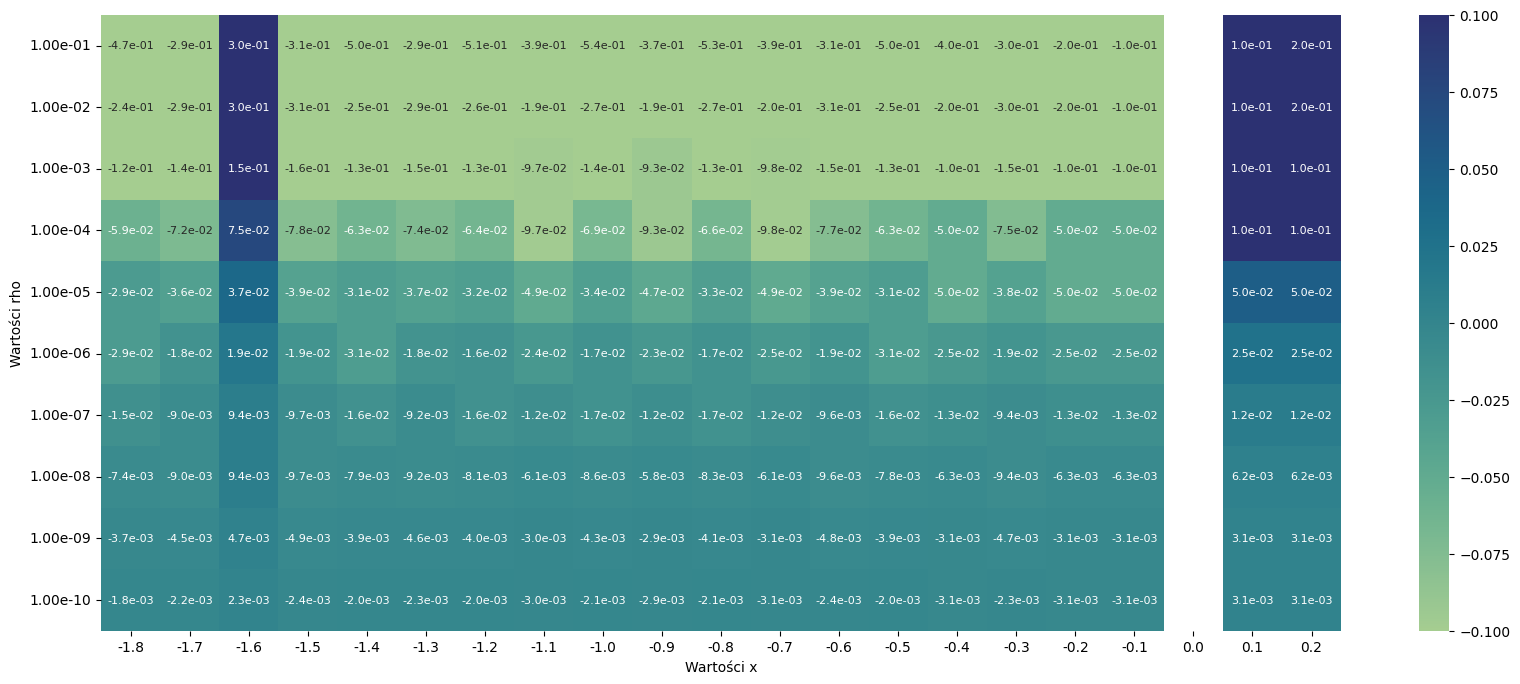
\includegraphics[width=\textwidth]{heatmap01.png}
  \end{minipage}
  \caption{Wykres wartości pierwiastka w zależności od \(\rho\) i \(x\)}
\end{figure}

\begin{figure}[H]
  \centering
  \begin{minipage}[b]{\textwidth}
    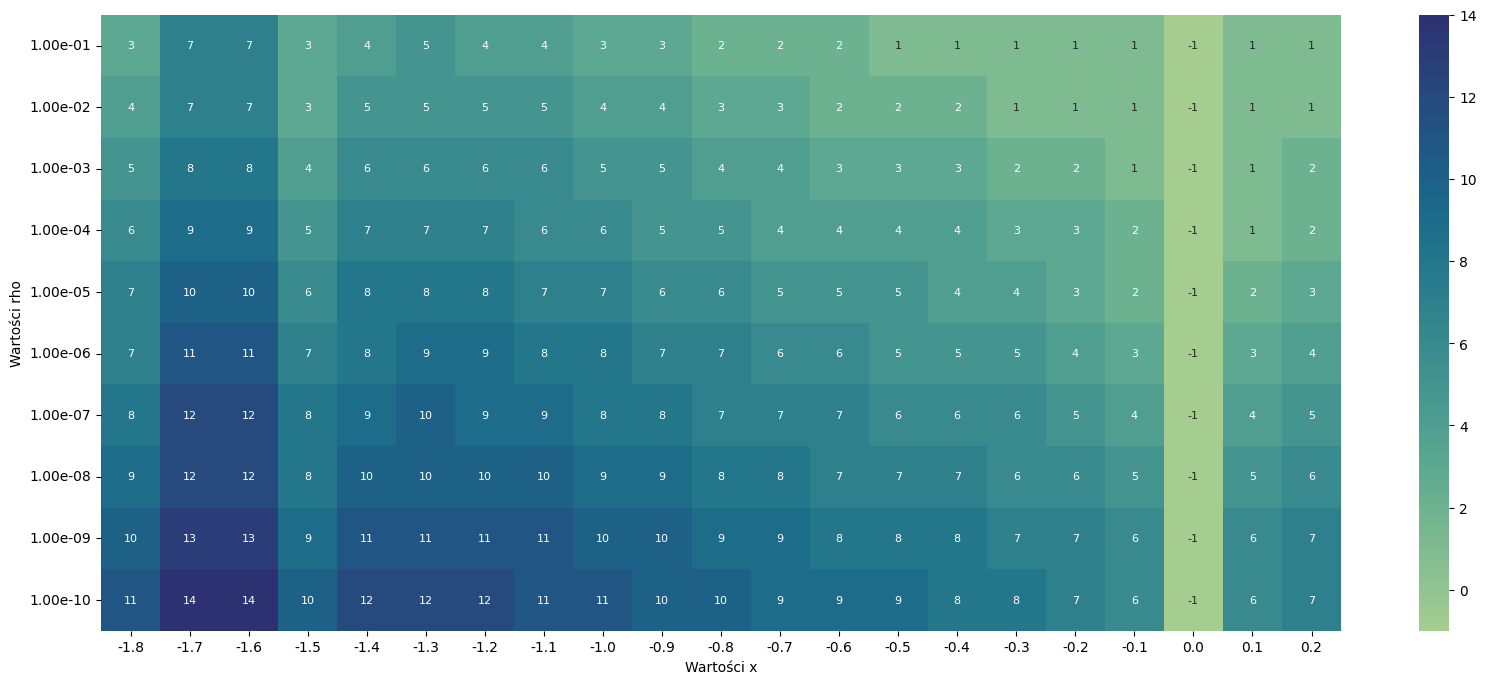
\includegraphics[width=\textwidth]{heatmap02.png}
  \end{minipage}
  \caption{Wykres liczby iteracji w zależności od \(\rho\) i \(x\)}
\end{figure}

\noindent
W poniższej tabeli przedstawiona została najlepsza otrzymana wartość przybliżenia (Oraz liczba iteracji, \(\rho\) i początkowe x dla którego została otrzymana) dla danych wartości prametru \(\rho\) oraz kryterium stopu w zestaweniu z prawdziwą wartością pierwiastka.

\begin{table}[H]
    \centering
    \begin{tabular}{|l|l|}
    \hline
        Prawdziwa wartość pierwiastka & 0.0 \\ \hline
        Najlepsze przybliżenie & -1.8e-03 \\ \hline
        Liczba iteracji & 11 \\ \hline
        Wartość $\rho$ & 1.0e-10 \\ \hline
        Wartość początkowa x & -1.8 \\ \hline
    \end{tabular}
\end{table}


\subsubsection{Kryterium wartości bezwzględnej wartości funkcji, \(\rho \in [10^{-11}, \ 10^{-20}]\)}

Na poniższych wykresach doskonale widać, że zmniejszenie wartości parametru \(\rho\) prowadzi w każdym przypadku do zwiększenia dokładności oraz liczby iteracji. Ponownie widać, że wybierając coraz bardziej oddalone punkty od prawdziej wartości pierwiastka otrzymujemy coraz większa liczbę iteracji. 

\begin{figure}[H]
  \centering
  \begin{minipage}[b]{\textwidth}
    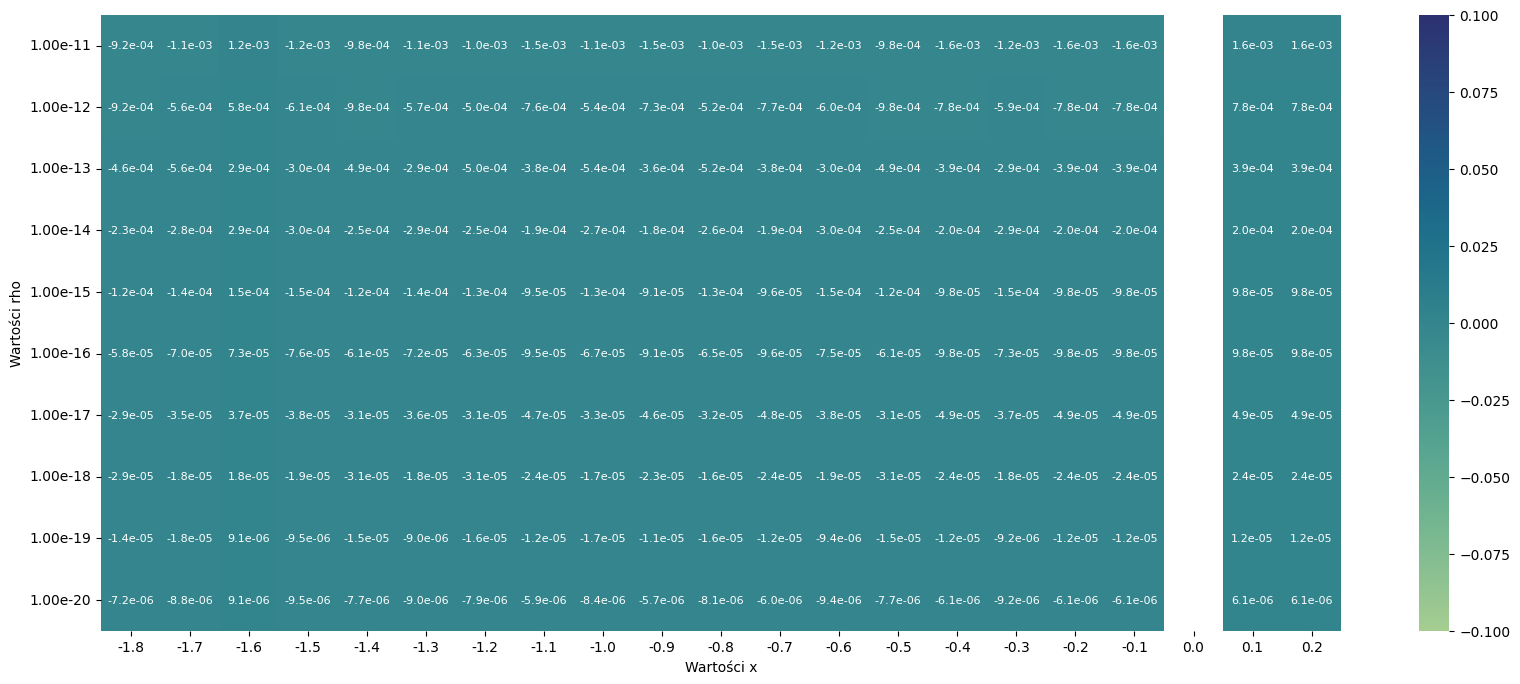
\includegraphics[width=\textwidth]{heatmap03.png}
    \caption{Wykres wartości pierwiastka w zależności od \(\rho\) i \(x\)}
  \end{minipage}
  
\end{figure}

\begin{figure}[H]
  \centering
  \begin{minipage}[b]{\textwidth}
    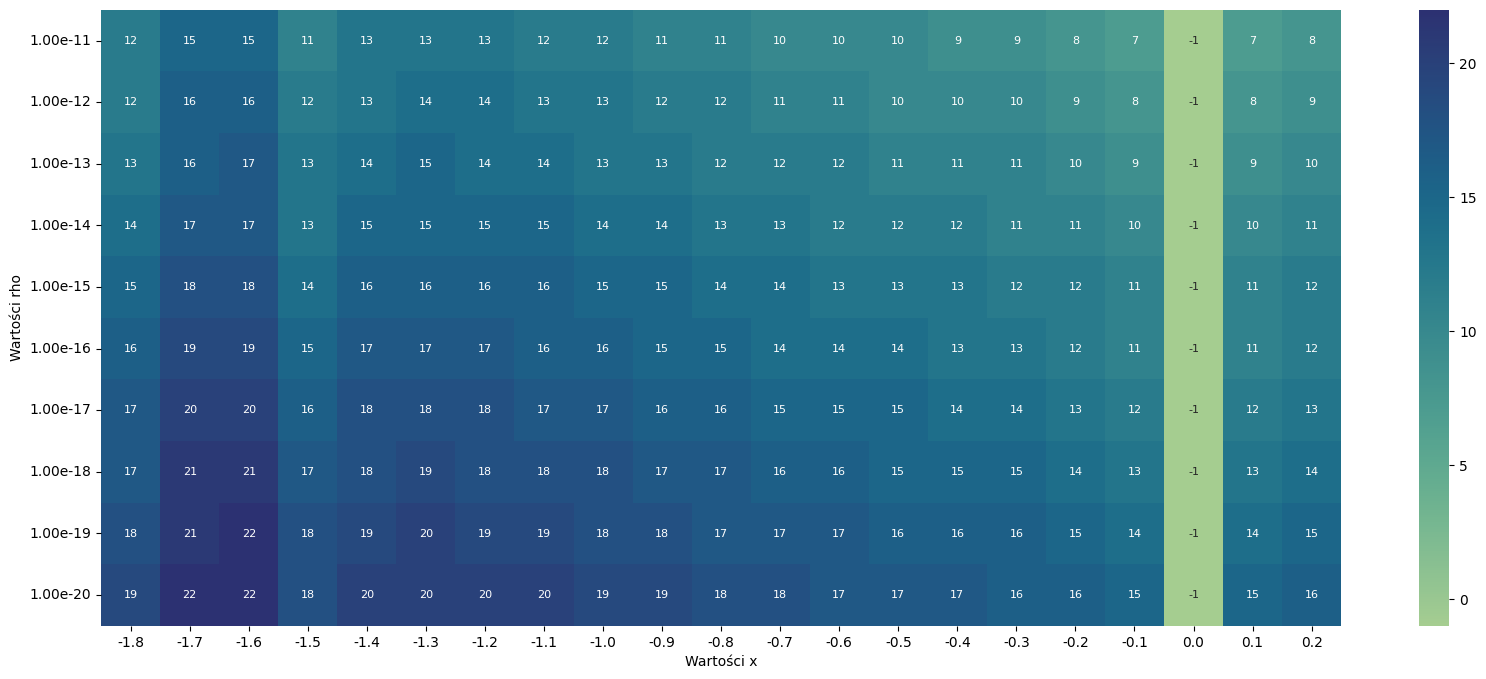
\includegraphics[width=\textwidth]{heatmap04.png}
  \end{minipage}
  \caption{Wykres liczby iteracji w zależności od \(\rho\) i \(x\)}
\end{figure}

\noindent
W poniższej tabeli przedstawiona została najlepsza otrzymana wartość przybliżenia (Oraz liczba iteracji, \(\rho\) i początkowe x dla którego została otrzymana) dla danych wartości prametru \(\rho\) oraz kryterium stopu w zestaweniu z prawdziwą wartością pierwiastka.

\begin{table}[H]
    \centering
    \begin{tabular}{|l|l|}
    \hline
        Prawdziwa wartość pierwiastka & 0.0 \\ \hline
        Najlepsze przybliżenie & -5.7e-06 \\ \hline
        Liczba iteracji & 19 \\ \hline
        Wartość $\rho$ & 1.0e-20 \\ \hline
        Wartość początkowa x & -0.9 \\ \hline
    \end{tabular}
\end{table}

\subsubsection{Wartość bezwzględna różnicy dwóch ostatnich przybliżeń pierwiastka, \(\rho \in [10^{-1}, \ 10^{-10}]\)}

Jak widać, w tym przypadku sytuacja jest bardzo podobna. Również otrzymujemy dobre przybliżenie pierwiastka, jednak liczba potrzebnych iteracji jest niemal dwukrotnie większa, niż w przypadku krytrium stopu związageo z wartością bezwzględną wartości funkcji. Ponownie liczba iteracji zwiększa się wraz z wzrostem odległości od pierwiastka

\begin{figure}[H]
  \centering
  \begin{minipage}[b]{\textwidth}
    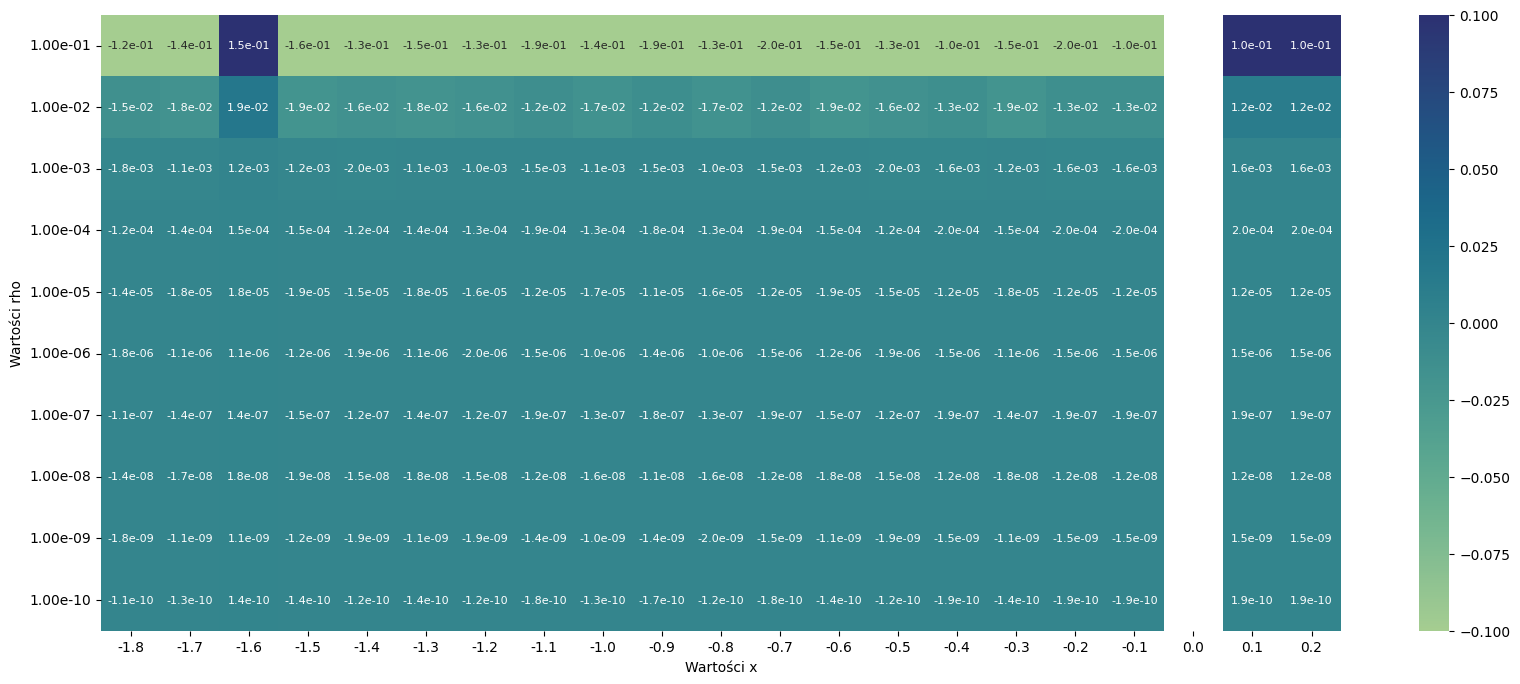
\includegraphics[width=\textwidth]{heatmap05.png}
    \caption{Wykres wartości pierwiastka w zależności od \(\rho\) i \(x\)}
  \end{minipage}
\end{figure}

\begin{figure}[H]
  \centering
  \begin{minipage}[b]{\textwidth}
    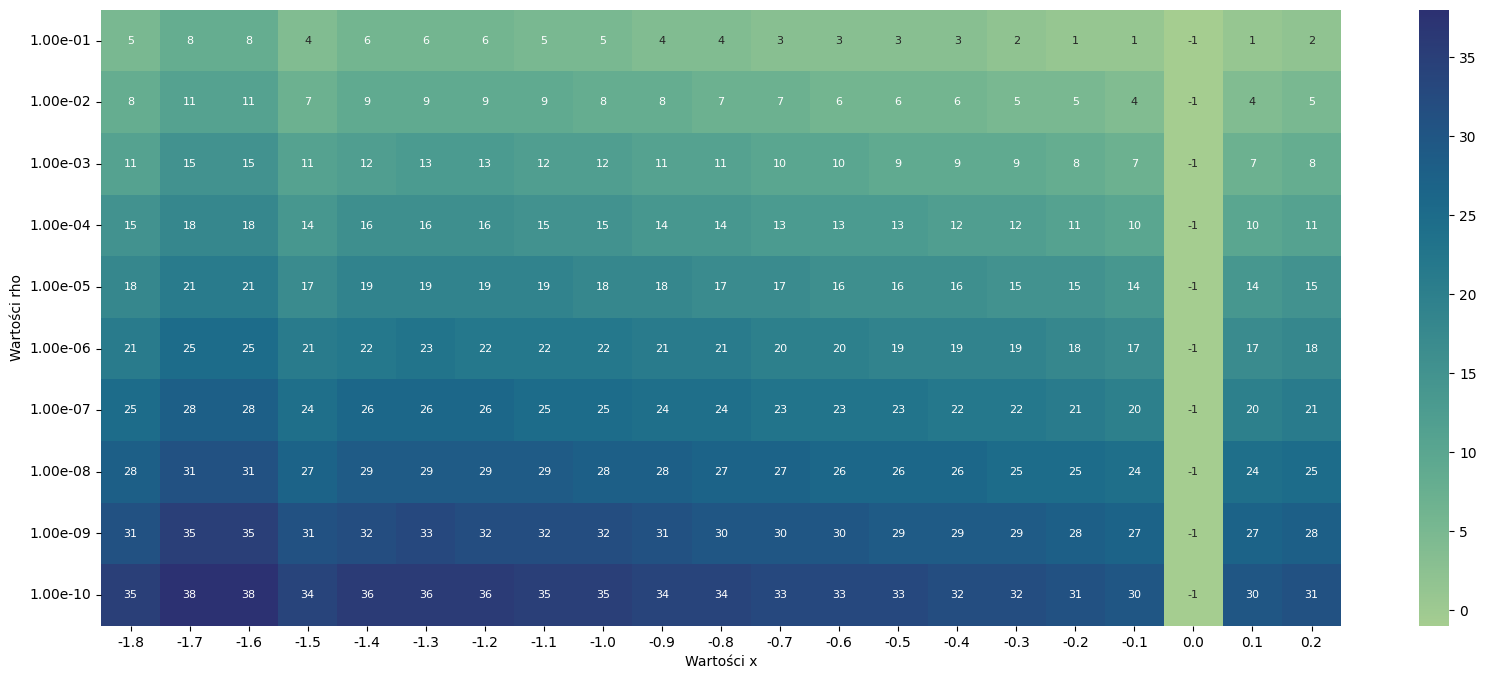
\includegraphics[width=\textwidth]{heatmap06.png}
  \end{minipage}
  \caption{Wykres liczby iteracji w zależności od \(\rho\) i \(x\)}
\end{figure}

\noindent
W poniższej tabeli przedstawiona została najlepsza otrzymana wartość przybliżenia (Oraz liczba iteracji, \(\rho\) i początkowe x dla którego została otrzymana) dla danych wartości prametru \(\rho\) oraz kryterium stopu w zestaweniu z prawdziwą wartością pierwiastka.

\begin{table}[H]
    \centering
    \begin{tabular}{|l|l|}
    \hline
        Prawdziwa wartość pierwiastka & 0.0 \\ \hline
        Najlepsze przybliżenie & -1.1e-10 \\ \hline
        Liczba iteracji & 35 \\ \hline
        Wartość $\rho$ & 1.0e-10 \\ \hline
        Wartość początkowa x & -1.8 \\ \hline
    \end{tabular}
\end{table}

\subsubsection{Wartość bezwzględna różnicy dwóch ostatnich przybliżeń pierwiastka, \(\rho \in [10^{-11}, \ 10^{-20}]\)}

Ponownie na poniższych wykresach doskonale widać, że zmniejszenie wartości parametru \(\rho\) prowadzi w każdym przypadku do zwiększenia dokładności oraz liczby iteracj oraz że wybierając coraz bardziej oddalone punkty od prawdziej wartości pierwiastka otrzymujemy coraz większa liczbę iteracji. 


\begin{figure}[H]
  \centering
  \begin{minipage}[b]{\textwidth}
    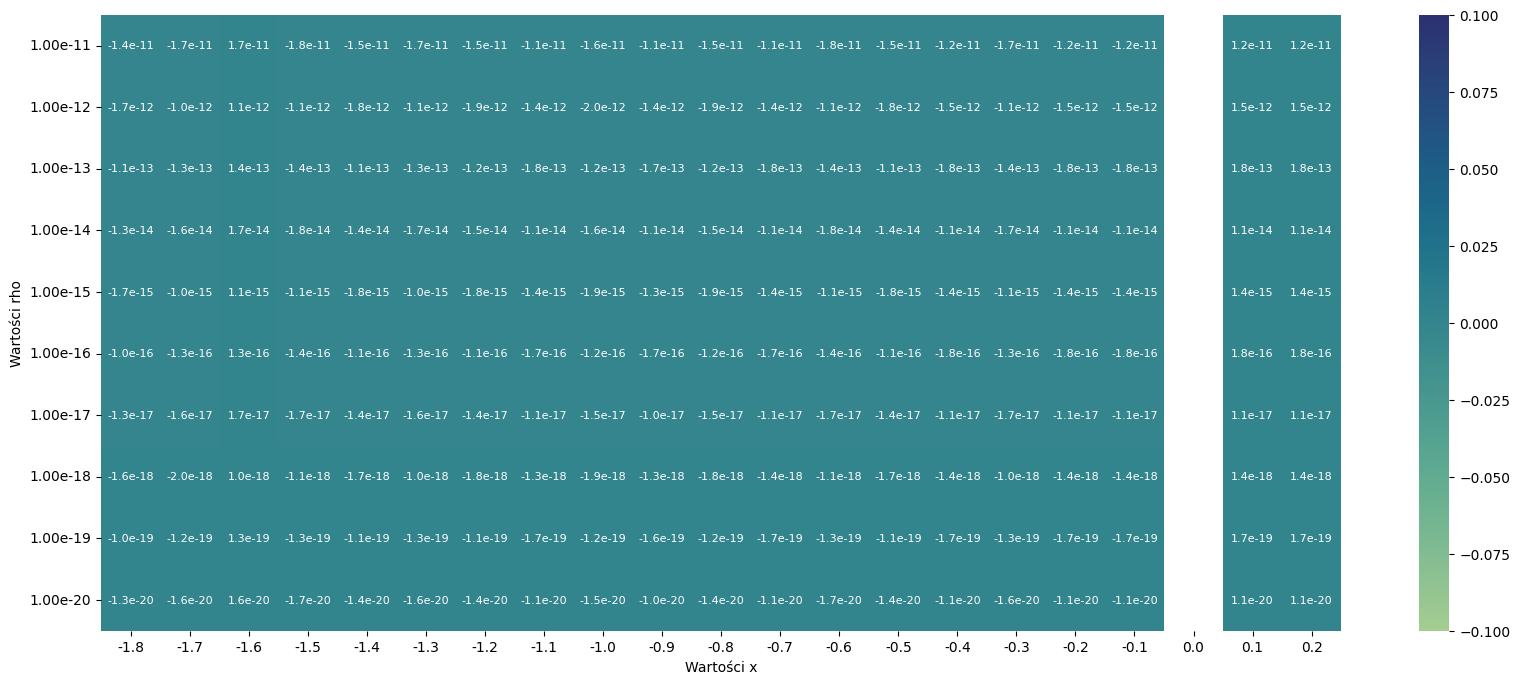
\includegraphics[width=\textwidth]{heatmap07.png}
  \end{minipage}
  \caption{Wykres wartości pierwiastka w zależności od \(\rho\) i \(x\)}
\end{figure}

\begin{figure}[H]
  \centering
  \begin{minipage}[b]{\textwidth}
    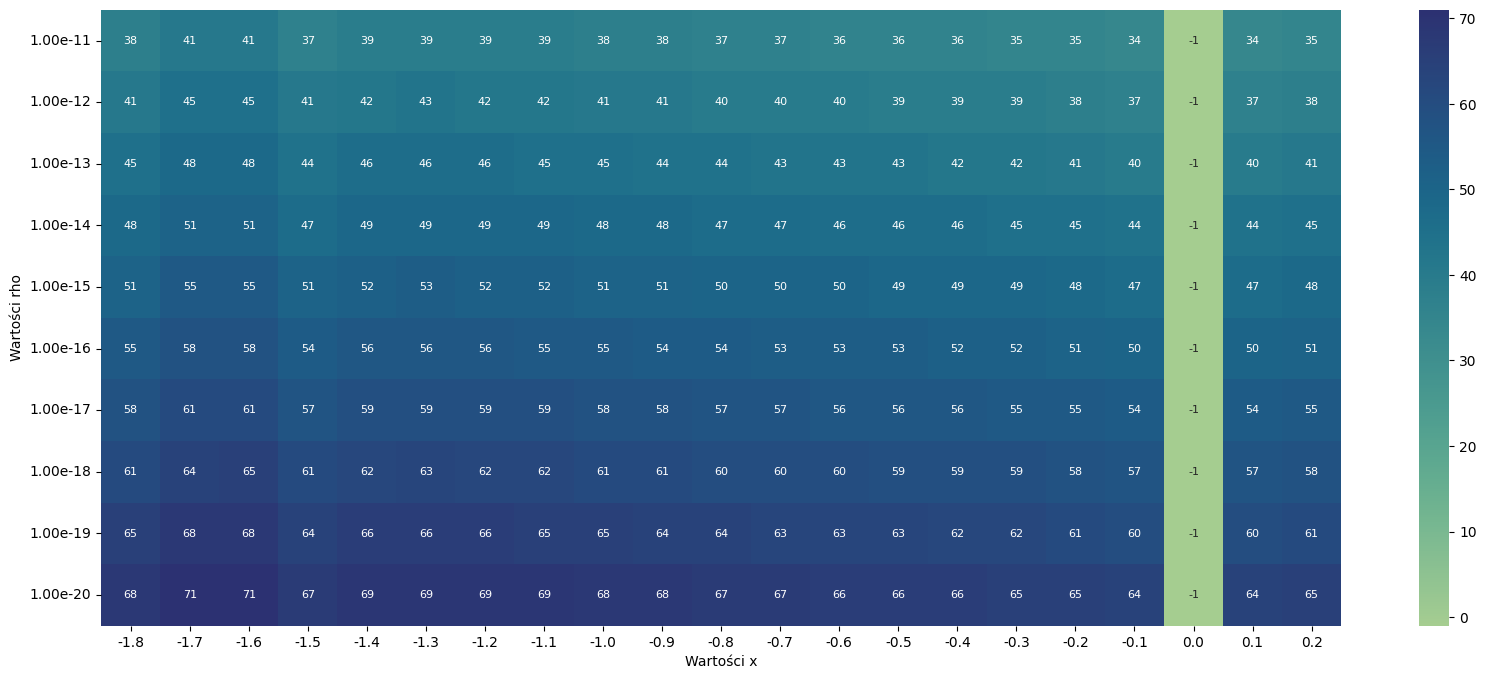
\includegraphics[width=\textwidth]{heatmap08.png}
  \end{minipage}
  \caption{Wykres liczby iteracji w zależności od \(\rho\) i \(x\)}
\end{figure}

\noindent
W poniższej tabeli przedstawiona została najlepsza otrzymana wartość przybliżenia (Oraz liczba iteracji, \(\rho\) i początkowe x dla którego została otrzymana) dla danych wartości prametru \(\rho\) oraz kryterium stopu w zestaweniu z prawdziwą wartością pierwiastka.

\begin{table}[H]
    \centering
    \begin{tabular}{|l|l|}
    \hline
        Prawdziwa wartość pierwiastka & 0.0 \\ \hline
        Najlepsze przybliżenie & -1.0e-20 \\ \hline
        Liczba iteracji & 69 \\ \hline
        Wartość $\rho$ & 1.0e-20 \\ \hline
        Wartość początkowa x & -0.9 \\ \hline
    \end{tabular}
\end{table}

\newpage

\subsection{Wyniki dla metody siecznych\textit{}}

Wyniki zostały podzielone ze względu na kryterium stopu oraz wartości parametru \(\rho\). Poza tym, w każdym przypadku jeden z początków przedziału stanowi początek lub koniec [a, b], a drugi \(x \in [-1.8, 0.2]\). Z uwagi na to, że za każdym razem dla przedziału, który kończy lub zaczyna od 0.0 otrzymuję dokładną wartość pierwiastka. Pominąłęm przy szukaniu najlepszego przybliżenia i w tabelach pod mapami cieplnymi pokazane są drugie najlepsze przybliżenia.

\subsubsection{Kryterium wartości bezwzględnej wartości funkcji, \(\rho \in [10^{-1}, 10^{-10}]\), początek przedziału ustalony na -1.8}

Jak widać na poniższym wykresie wszystkie wartości są bardzo zbliżone do szukanego pierwiastka. Natomiast z uwagi na specyfikę funkcji tj. \(f(0) = 0\), dla przedziału \([-1.8, 0.0]\) otrzymujemy dokładny wynik w pierwszej iteracji.

\begin{figure}[H]
  \centering
  \begin{minipage}[b]{\textwidth}
    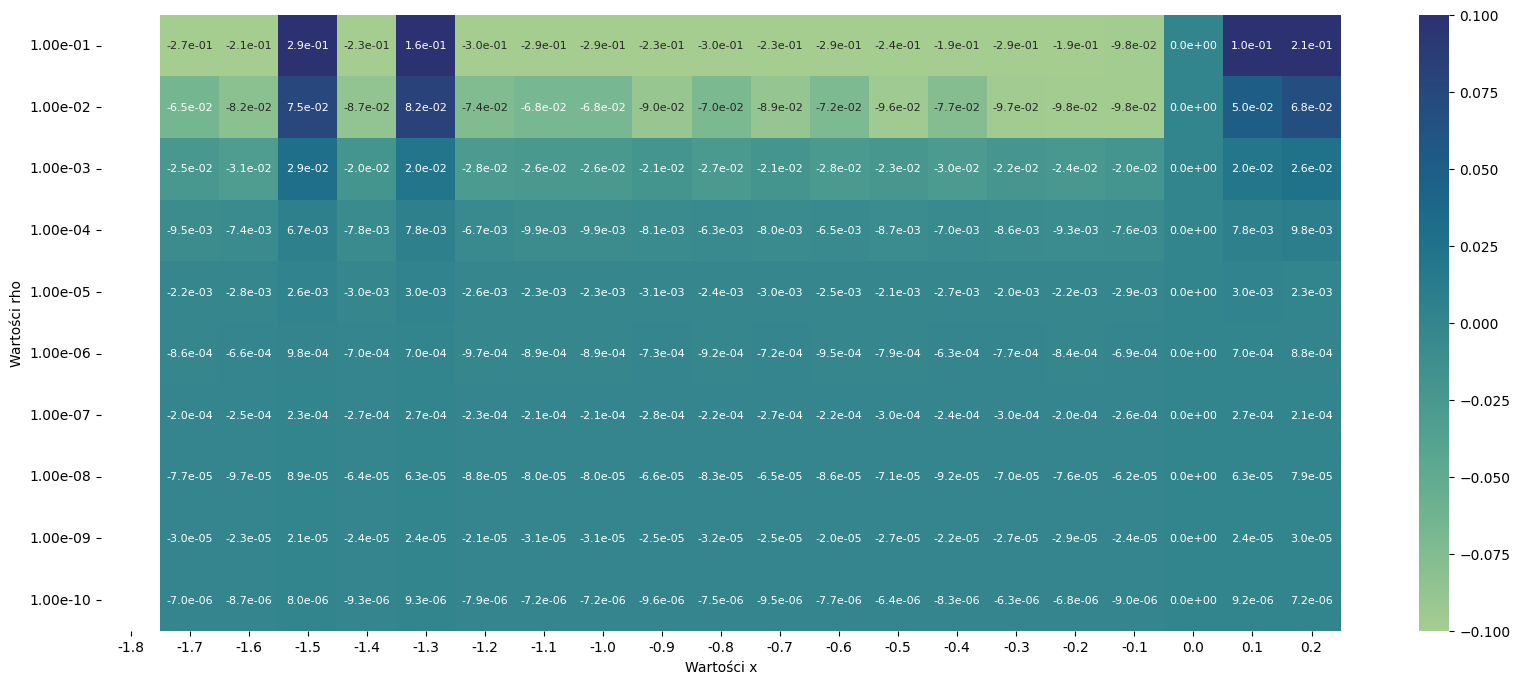
\includegraphics[width=\textwidth]{heatmap09.png}
  \end{minipage}
  \caption{Wykres wartości pierwiastka w zależności od \(\rho\) i \(x\)}
\end{figure}

\begin{figure}[H]
  \centering
  \begin{minipage}[b]{\textwidth}
    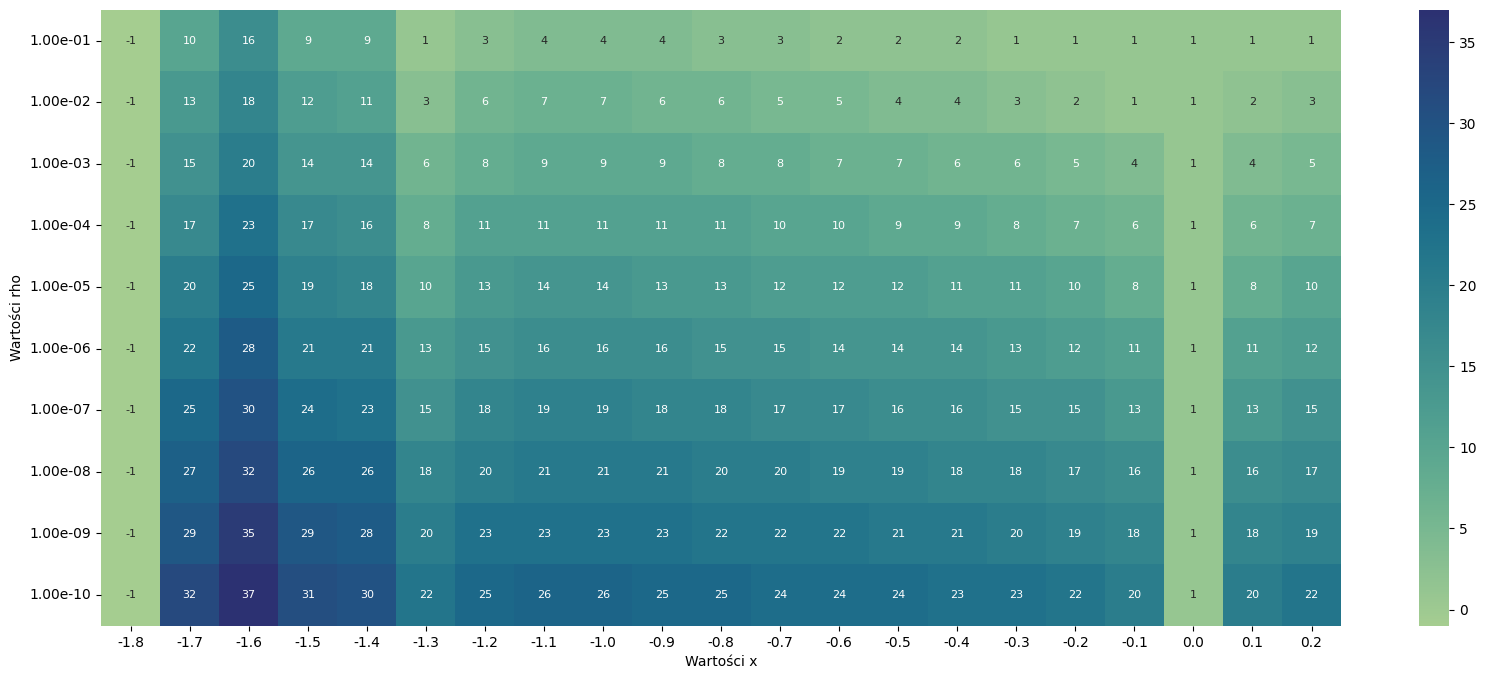
\includegraphics[width=\textwidth]{heatmap10.png}
  \end{minipage}
  \caption{Wykres liczby iteracji w zależności od \(\rho\) i \(x\)}
\end{figure}

\noindent
W tabli poniżej przedstawiona została druga najlepsza otrzymana wartość przybliżenia (Oraz liczba iteracji, \(\rho\) i początkowe x dla którego została otrzymana) dla danych wartości prametru \(\rho\) oraz kryterium stopu w zestaweniu z prawdziwą wartością pierwiastka.

\begin{table}[H]
    \centering
    \begin{tabular}{|l|l|}
    \hline
        Prawdziwa wartość pierwiastka & 0.0 \\ \hline
        Najlepsze przybliżenie & -6.3e-06 \\ \hline
        Liczba iteracji & 23 \\ \hline
        Wartość $\rho$ & 1.0e-10 \\ \hline
        Początek przedziału & -1.8 \\ \hline
        Koniec przedziału & -0.3 \\ \hline
    \end{tabular}
    \caption{Wartość drugiego najlepszego przybliżenia}
\end{table}

\subsubsection{Kryterium wartości bezwzględnej wartości funkcji, \(\rho \in [10^{-11}, 10^{-20}]\), początek przedziału ustalony na -1.8}

Ponownie zmniejszenie wartości \(\rho\) prowadzi do otrzymania lepszego przybliżenia (poza punktem 0.0).

\begin{figure}[H]
  \centering
  \begin{minipage}[b]{\textwidth}
    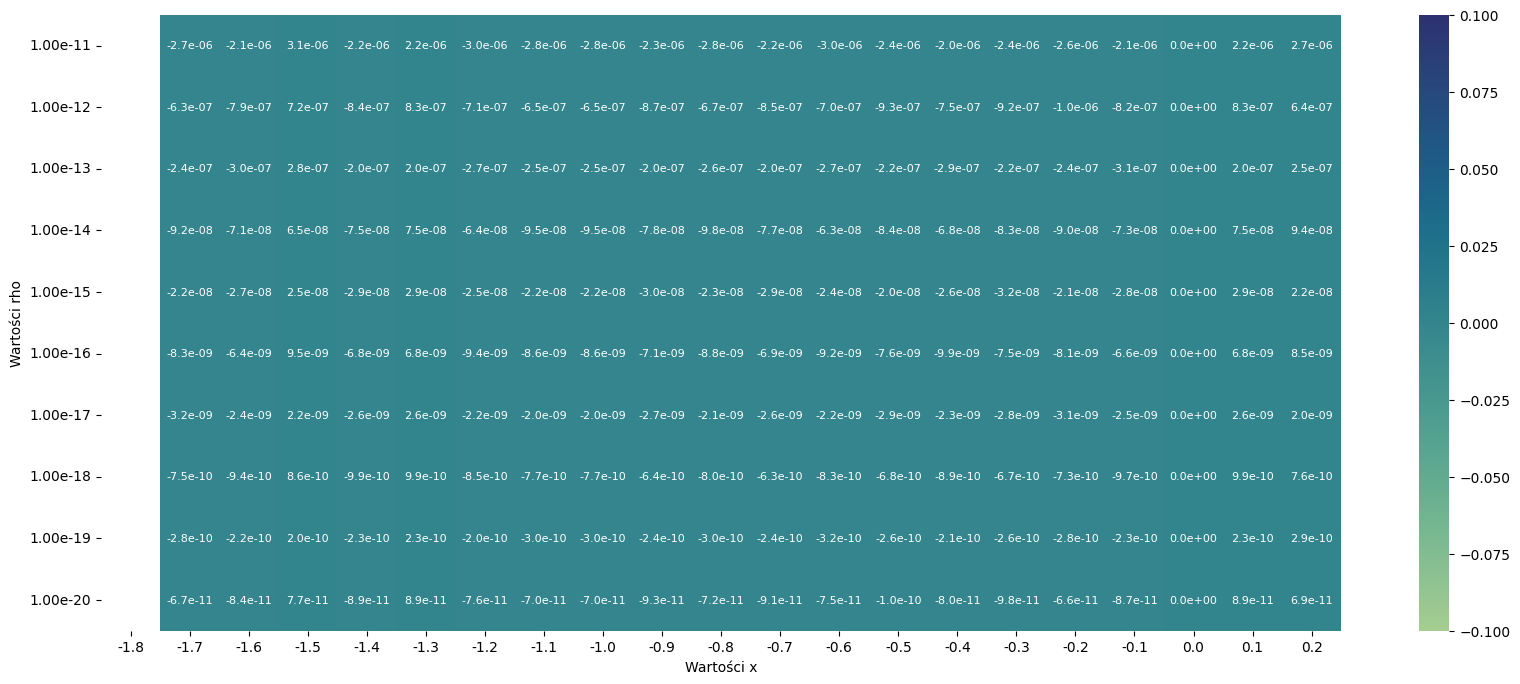
\includegraphics[width=\textwidth]{heatmap11.png}
  \end{minipage}
  \caption{Wykres wartości pierwiastka w zależności od \(\rho\) i \(x\)}
\end{figure}

\begin{figure}[H]
  \centering
  \begin{minipage}[b]{\textwidth}
    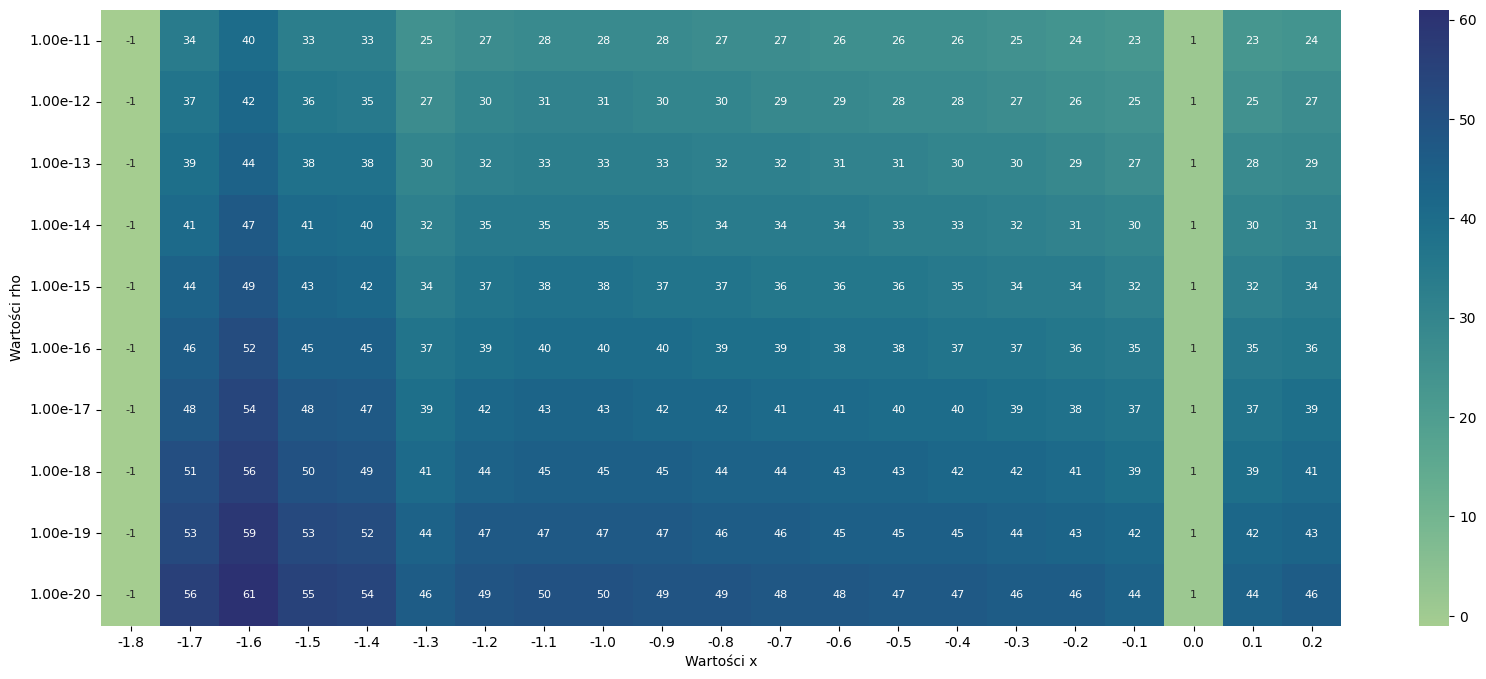
\includegraphics[width=\textwidth]{heatmap12.png}
  \end{minipage}
  \caption{Wykres liczby iteracji w zależności od \(\rho\) i \(x\)}
\end{figure}

\noindent
W tabli poniżej przedstawiona została druga najlepsza otrzymana wartość przybliżenia (Oraz liczba iteracji, \(\rho\) i początkowe x dla którego została otrzymana) dla danych wartości prametru \(\rho\) oraz kryterium stopu w zestaweniu z prawdziwą wartością pierwiastka.

\begin{table}[H]
    \centering
    \begin{tabular}{|l|l|}
    \hline
        Prawdziwa wartość pierwiastka & 0.0 \\ \hline
        Najlepsze przybliżenie & -6.6e-11 \\ \hline
        Liczba iteracji & 46 \\ \hline
        Wartość $\rho$ & 1.0e-20 \\ \hline
        Początek przedziału & -1.8 \\ \hline
        Koniec przedziału & -0.2 \\ \hline
    \end{tabular}
    \caption{Wartość drugiego najlepszego przybliżenia}
\end{table}

\subsubsection{Kryterium wartości bezwzględnej wartości funkcji, \(\rho \in [10^{-1}, 10^{-10}]\), koniec przedziału ustalony na 0.2}

Otrzymane wyniki są bliskie szukanemu pierwiastkowi, a zmniejszenie parametru \(\rho\) prowadzi do zwiększenia dokładności. Ponownie najlepsze otrzymane przybliżenie jest tożsame z prawdziwą wartością pierwiastka.

\begin{figure}[H]
  \centering
  \begin{minipage}[b]{0.9\textwidth}
    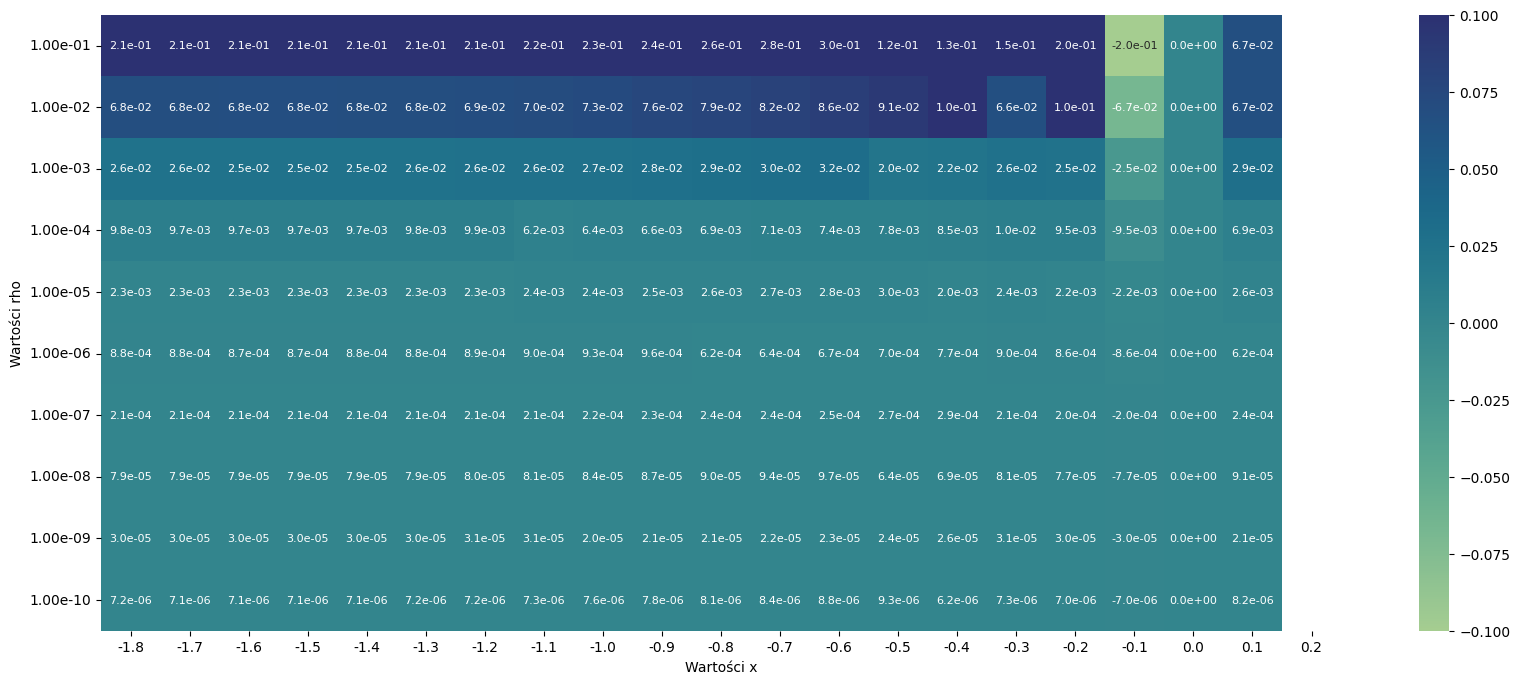
\includegraphics[width=\textwidth]{heatmap13.png}
  \end{minipage}
  \caption{Wykres wartości pierwiastka w zależności od \(\rho\) i \(x\)}
\end{figure}

\begin{figure}[H]
  \centering
  \begin{minipage}[b]{0.9\textwidth}
    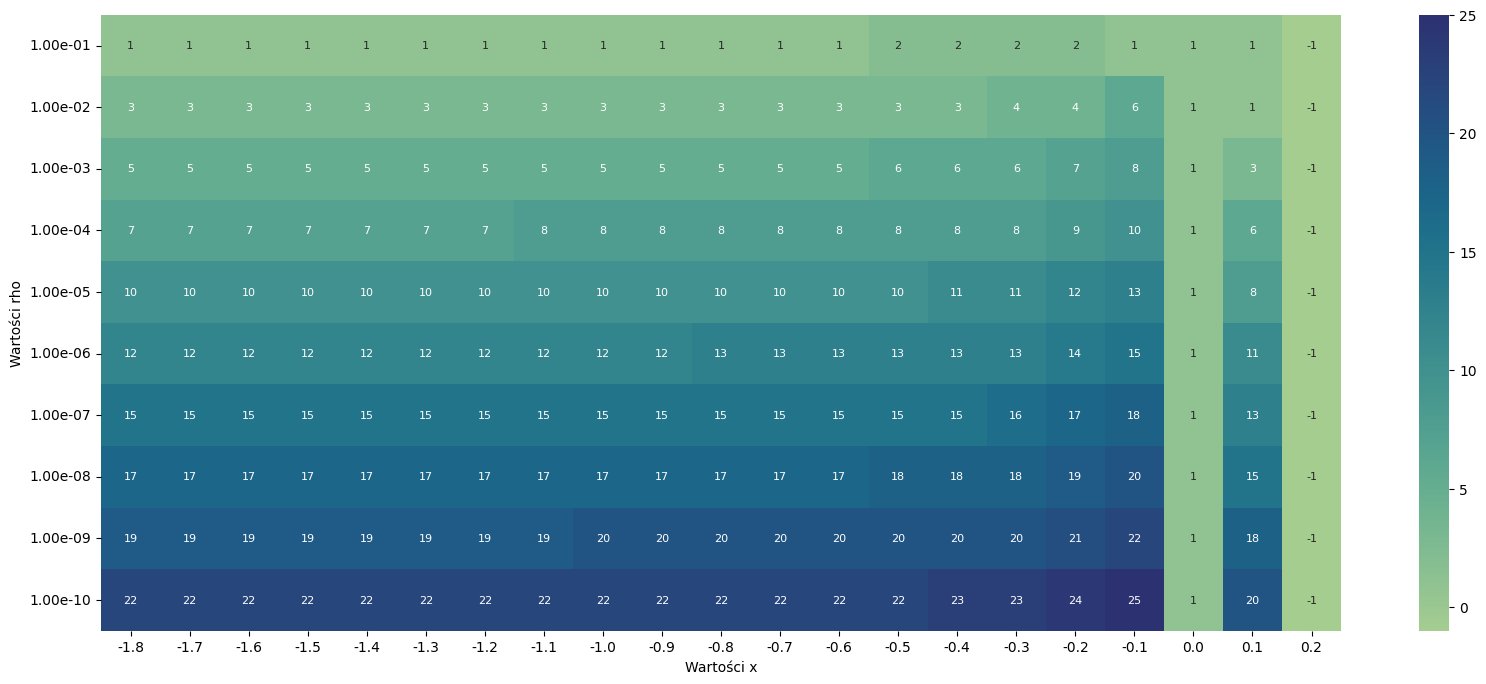
\includegraphics[width=\textwidth]{heatmap14.png}
  \end{minipage}
  \caption{Wykres liczby iteracji w zależności od \(\rho\) i \(x\)}
\end{figure}

\noindent
W tabli poniżej przedstawiona została druga najlepsza otrzymana wartość przybliżenia (Oraz liczba iteracji, \(\rho\) i początkowe x dla którego została otrzymana) dla danych wartości prametru \(\rho\) oraz kryterium stopu w zestaweniu z prawdziwą wartością pierwiastka.

\begin{table}[H]
    \centering
    \begin{tabular}{|l|l|}
    \hline
        Prawdziwa wartość pierwiastka & 0.0 \\ \hline
        Najlepsze przybliżenie & 6.2-06 \\ \hline
        Liczba iteracji & 26 \\ \hline
        Wartość $\rho$ & 1.0e-10 \\ \hline
        Początek przedziału & -0.4 \\ \hline
        Koniec przedziału & 0.2 \\ \hline
    \end{tabular}
    \caption{Wartość drugiego najlepszego przybliżenia}
\end{table}

\subsubsection{Kryterium wartości bezwzględnej, \(\rho \in [10^{-11}, 10^{-20}]\), koniec przedziału ustalony na 0.2}

Zmniejszenie parametru \(\rho\) znacznie polepszyło otrzymane przybliżenie. Jak widać na mapie cieplnej przybliżena się bardzo bliskie szukanemu pierwiastkowi.

\begin{figure}[H]
  \centering
  \begin{minipage}[b]{0.9\textwidth}
    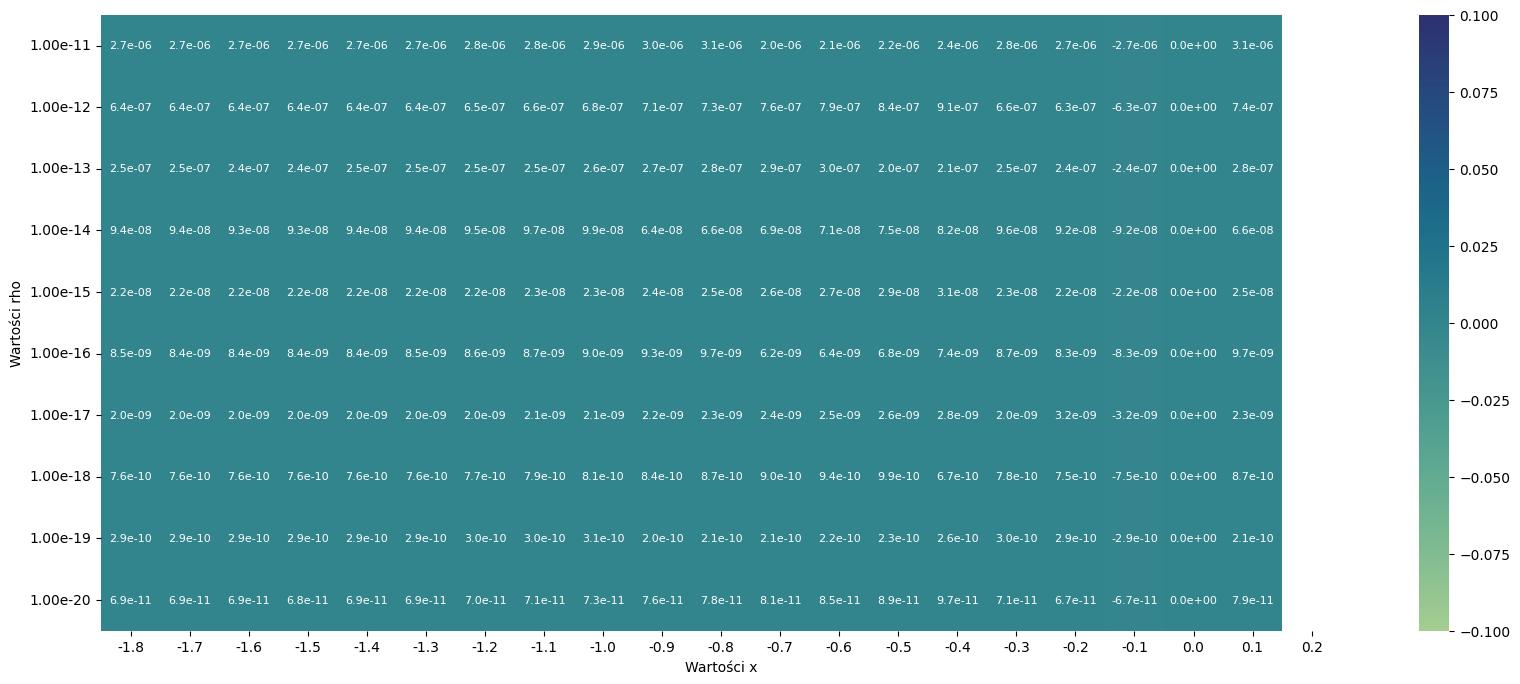
\includegraphics[width=\textwidth]{heatmap15.png}
  \end{minipage}
  \caption{Wykres wartości pierwiastka w zależności od \(\rho\) i \(x\)}
\end{figure}

\begin{figure}[H]
  \centering
  \begin{minipage}[b]{0.9\textwidth}
    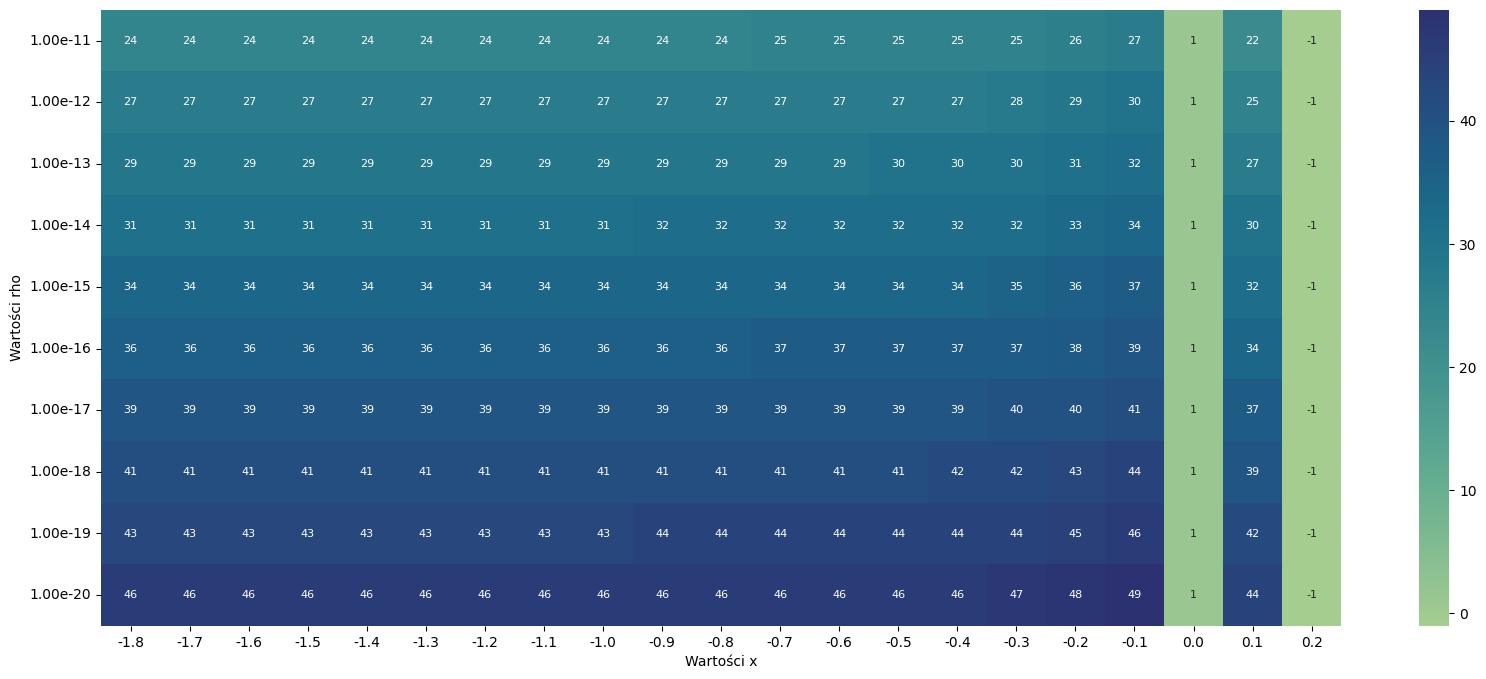
\includegraphics[width=\textwidth]{heatmap16.png}
  \end{minipage}
  \caption{Wykres liczby iteracji w zależności od \(\rho\) i \(x\)}
\end{figure}

\noindent
W tabli poniżej przedstawiona została druga najlepsza otrzymana wartość przybliżenia (Oraz liczba iteracji, \(\rho\) i początkowe x dla którego została otrzymana) dla danych wartości prametru \(\rho\) oraz kryterium stopu w zestaweniu z prawdziwą wartością pierwiastka.

\begin{table}[H]
    \centering
    \begin{tabular}{|l|l|}
    \hline
        Prawdziwa wartość pierwiastka & 0.0 \\ \hline
        Najlepsze przybliżenie & 6.7-11 \\ \hline
        Liczba iteracji & 48 \\ \hline
        Wartość $\rho$ & 1.0e-20 \\ \hline
        Początek przedziału & -0.2 \\ \hline
        Koniec przedziału & 0.2 \\ \hline
    \end{tabular}
    \caption{Wartość drugiego najlepszego przybliżenia}
\end{table}

\subsubsection{Wartość bezwzględna różnicy dwóch ostatnich przybliżeń pierwiastka, \(\rho \in [10^{-1}, 10^{-10}]\), początek przedziału ustalony na -1.8}

Jak widać na poniższym wykresie wszystkie wartości są bliskie szukanemu pierwiastkowi, poza wartościami, gdzie \(\rho \in [1e-01, 1e-02]\). W tym przedzialem otrzymane przybliżenie jest dość słabe.

\begin{figure}[H]
  \centering
  \begin{minipage}[b]{0.9\textwidth}
    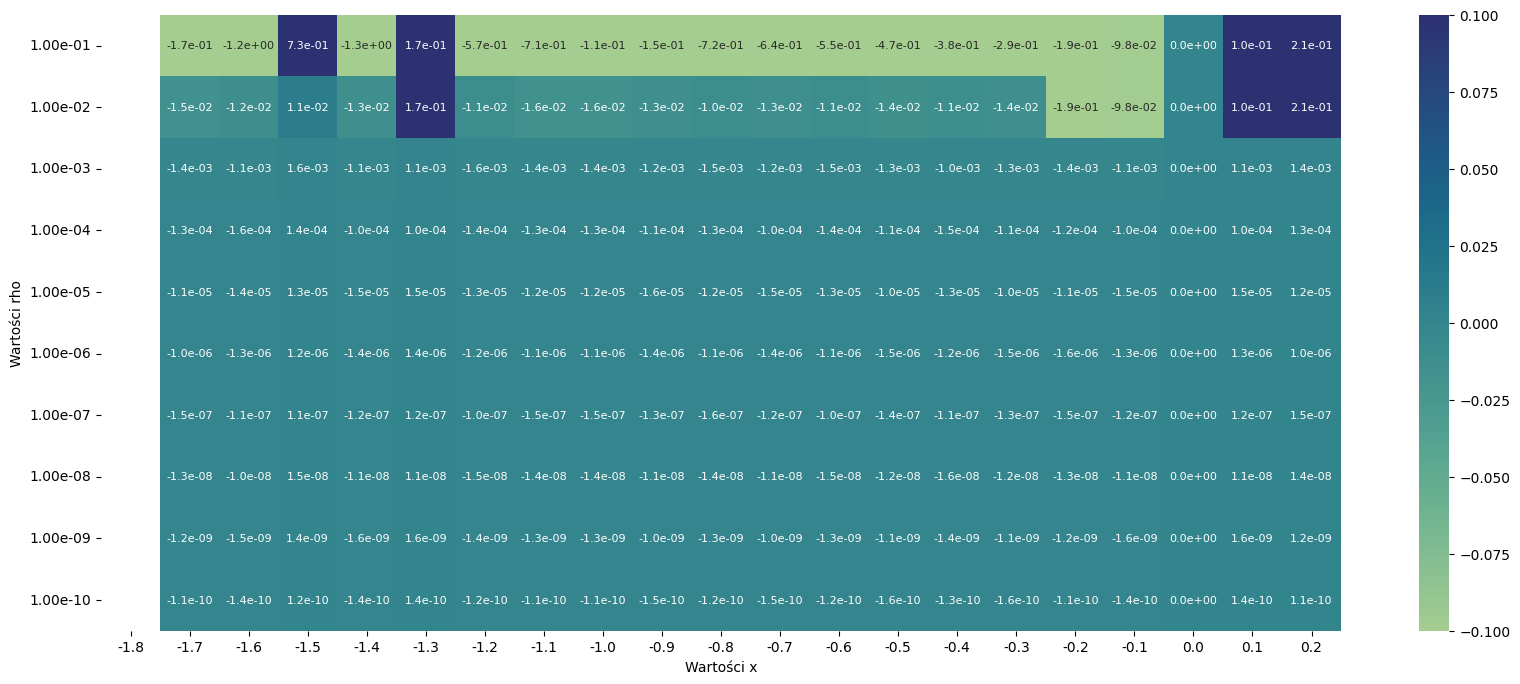
\includegraphics[width=\textwidth]{heatmap17.png}
  \end{minipage}
  \caption{Wykres wartości pierwiastka w zależności od \(\rho\) i \(x\)}
\end{figure}

\begin{figure}[H]
  \centering
  \begin{minipage}[b]{0.9\textwidth}
    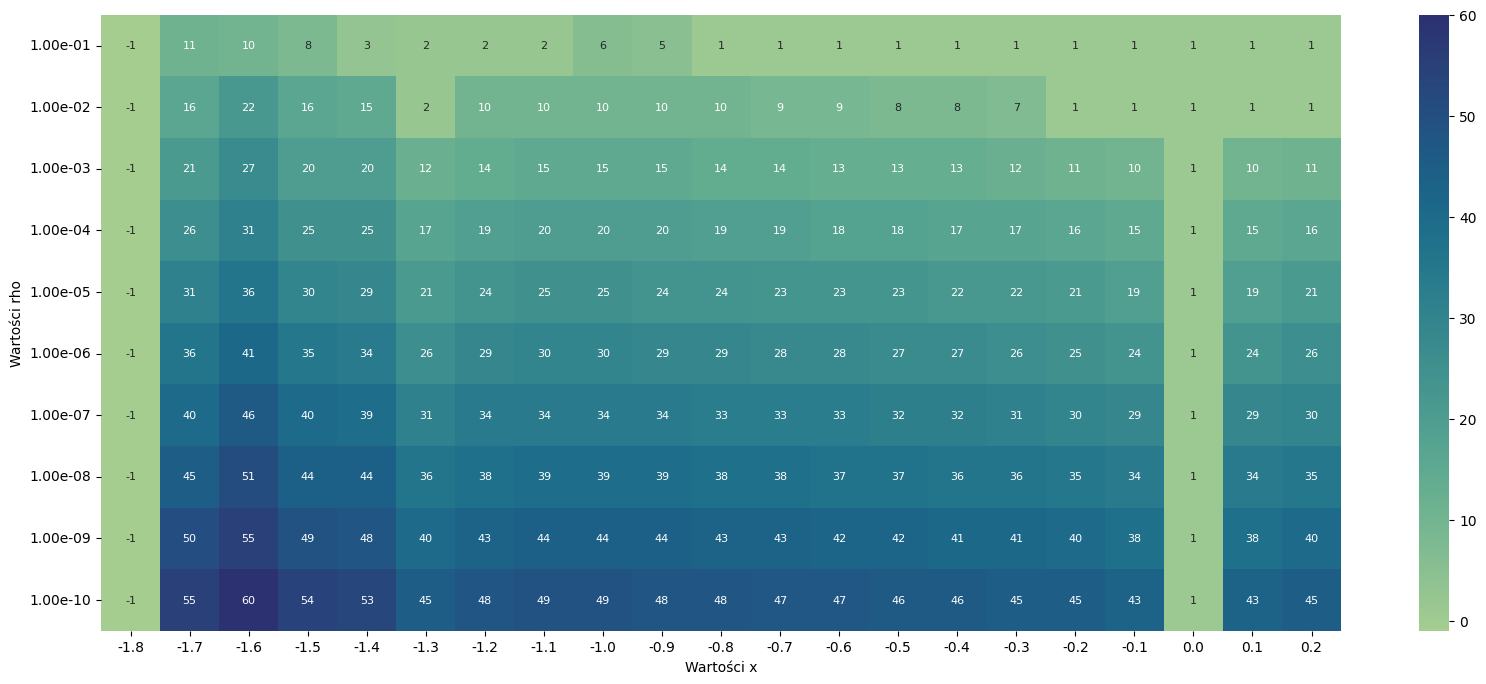
\includegraphics[width=\textwidth]{heatmap18.png}
  \end{minipage}
  \caption{Wykres liczby iteracji w zależności od \(\rho\) i \(x\)}
\end{figure}

\noindent
W tabli poniżej przedstawiona została druga najlepsza otrzymana wartość przybliżenia (Oraz liczba iteracji, \(\rho\) i początkowe x dla którego została otrzymana) dla danych wartości prametru \(\rho\) oraz kryterium stopu w zestaweniu z prawdziwą wartością pierwiastka.

\begin{table}[H]
    \centering
    \begin{tabular}{|l|l|}
    \hline
        Prawdziwa wartość pierwiastka & 0.0 \\ \hline
        Najlepsze przybliżenie & -1.1e-10 \\ \hline
        Liczba iteracji & 45 \\ \hline
        Wartość $\rho$ & 1.0e-10 \\ \hline
        Początek przedziału & -1.8 \\ \hline
        Koniec przedziału & -0.2 \\ \hline
    \end{tabular}
    \caption{Wartość drugiego najlepszego przybliżenia}
\end{table}

\subsubsection{Wartość bezwzględna różnicy dwóch ostatnich przybliżeń pierwiastka, \(\rho \in [10^{-11}, 10^{-20}]\), początek przedziału ustalony na -1.8}

Ponownie nie ma żadnych zaskoczeń, przybliżenie w każdym przypadku jest bardzo dobre i bliskie szukanej wartości.

\begin{figure}[H]
  \centering
  \begin{minipage}[b]{0.9\textwidth}
    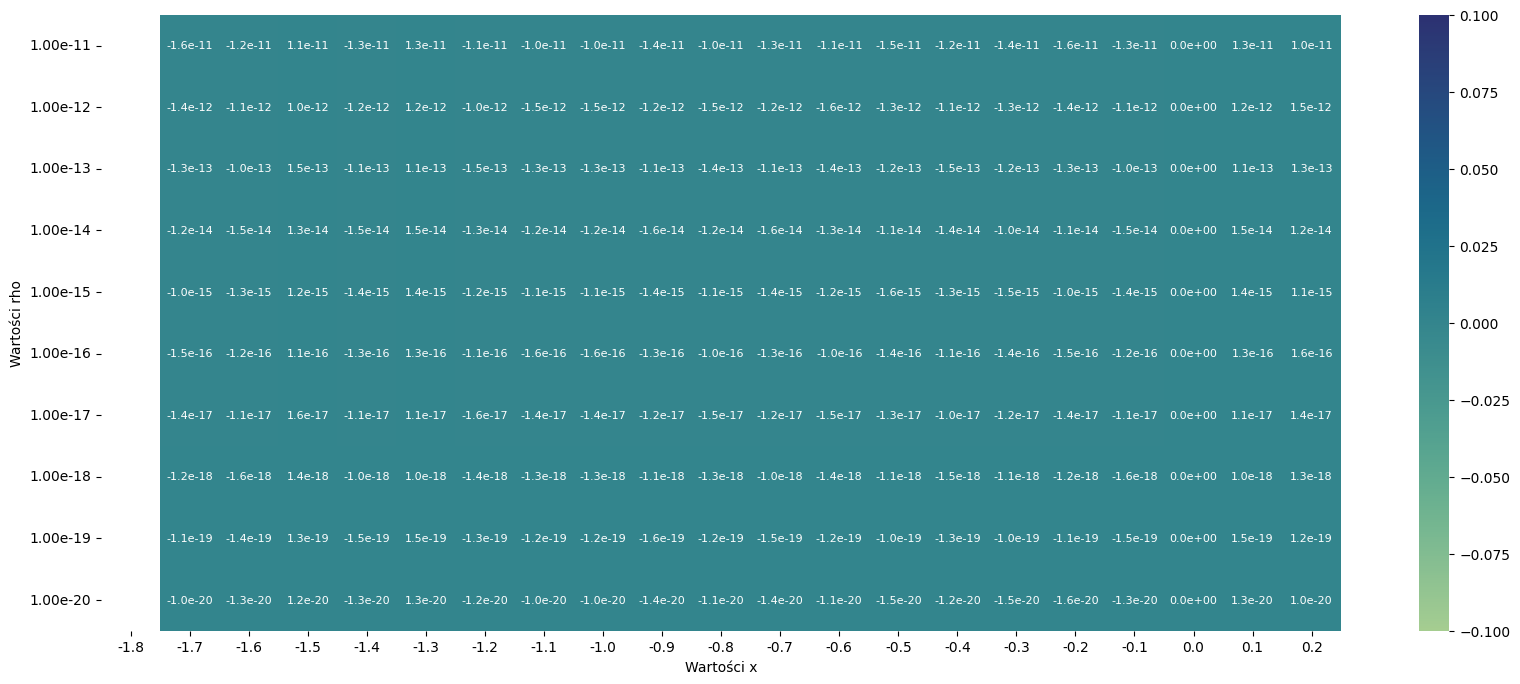
\includegraphics[width=\textwidth]{heatmap19.png}
  \end{minipage}
  \caption{Wykres wartości pierwiastka w zależności od \(\rho\) i \(x\)}
\end{figure}

\begin{figure}[H]
  \centering
  \begin{minipage}[b]{0.9\textwidth}
    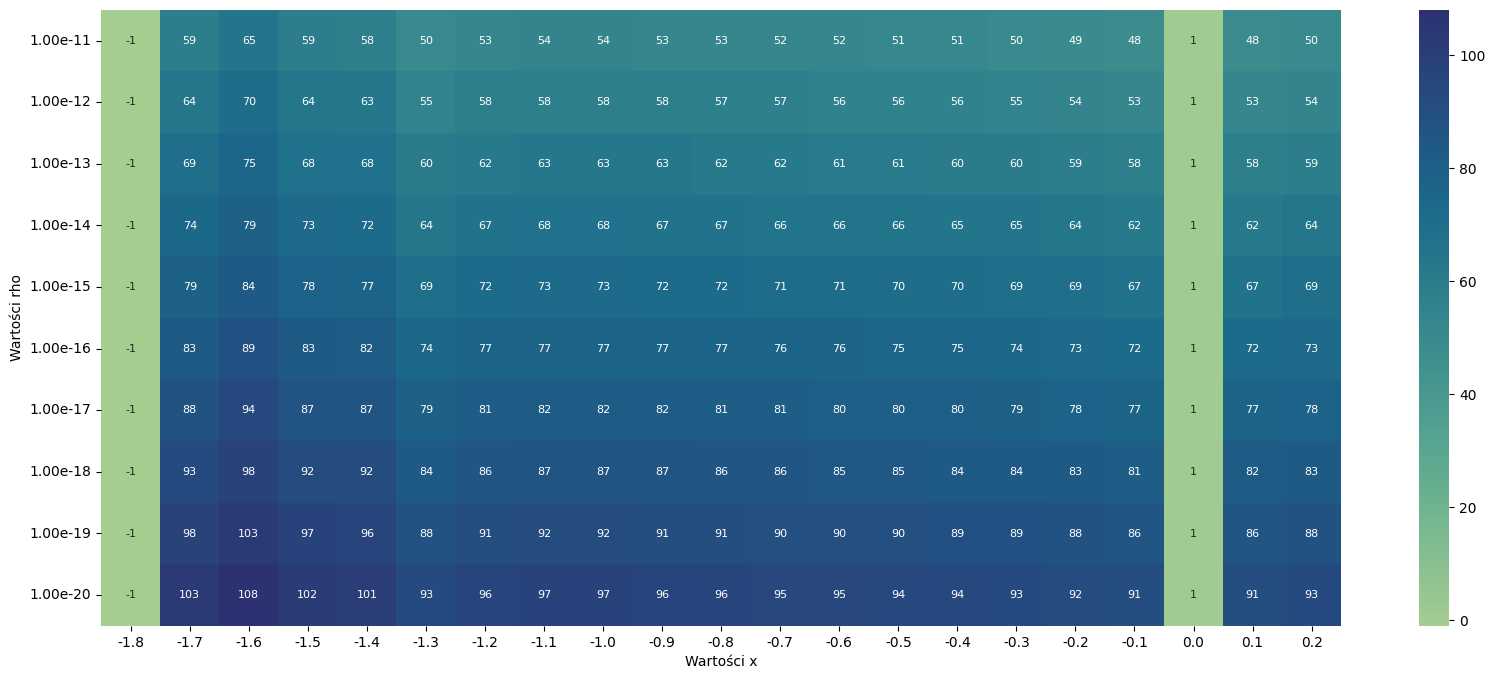
\includegraphics[width=\textwidth]{heatmap20.png}
  \end{minipage}
  \caption{Wykres liczby iteracji w zależności od \(\rho\) i \(x\)}
\end{figure}

\noindent
W tabli poniżej przedstawiona została druga najlepsza otrzymana wartość przybliżenia (Oraz liczba iteracji, \(\rho\) i początkowe x dla którego została otrzymana) dla danych wartości prametru \(\rho\) oraz kryterium stopu w zestaweniu z prawdziwą wartością pierwiastka.

\begin{table}[H]
    \centering
    \begin{tabular}{|l|l|}
    \hline
        Prawdziwa wartość pierwiastka & 0.0 \\ \hline
        Najlepsze przybliżenie & -1.0e-20 \\ \hline
        Liczba iteracji & 103 \\ \hline
        Wartość $\rho$ & 1.0e-20 \\ \hline
        Początek przedziału & -1.8 \\ \hline
        Koniec przedziału & -1.7 \\ \hline
    \end{tabular}
    \caption{Wartość drugiego najlepszego przybliżenia}
\end{table}

\subsubsection{Wartość bezwzględna różnicy dwóch ostatnich przybliżeń pierwiastka, \(\rho \in [10^{-1}, 10^{-10}]\), koniec przedziału ustalony na 0.2}

W tym przypadku, przy wybraniu początku przedziału jako \(-0.2\) lub \(-0.1\) i wartości \(\rho \in [1e-0.1, 1e08]\) przybliżenie jest bardzo złe podobnie dzieje się przy wybraniu poczatku przedziału jako liczbę z zakresu \([-1.8, -0.3]\) i \(\rho = 1e-01\) oraz początku przedziału z zakresu \([-1.8, -1.3]\) i \(\rho = 1e-02\).

\begin{figure}[H]
  \centering
  \begin{minipage}[b]{0.9\textwidth}
    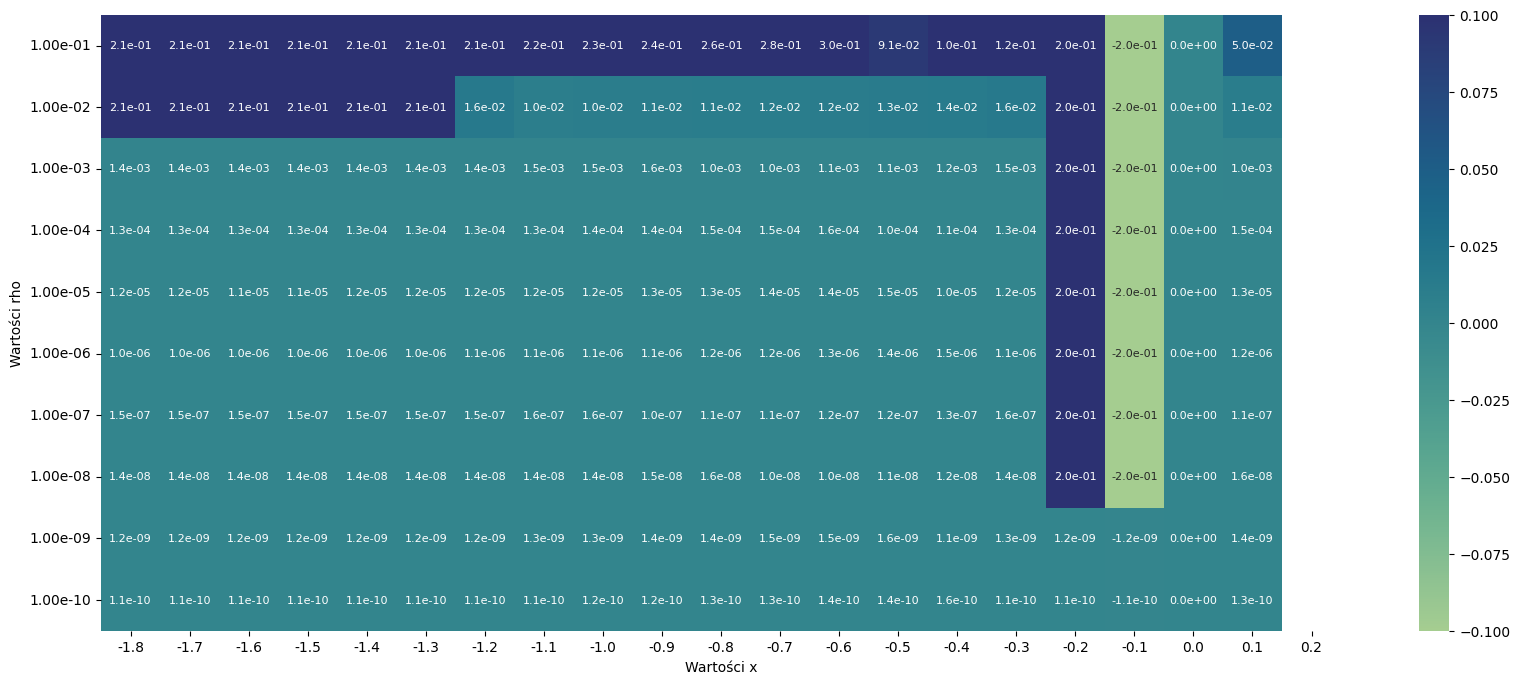
\includegraphics[width=\textwidth]{heatmap21.png}
  \end{minipage}
  \caption{Wykres wartości pierwiastka w zależności od \(\rho\) i \(x\)}
\end{figure}

\begin{figure}[H]
  \centering
  \begin{minipage}[b]{0.9\textwidth}
    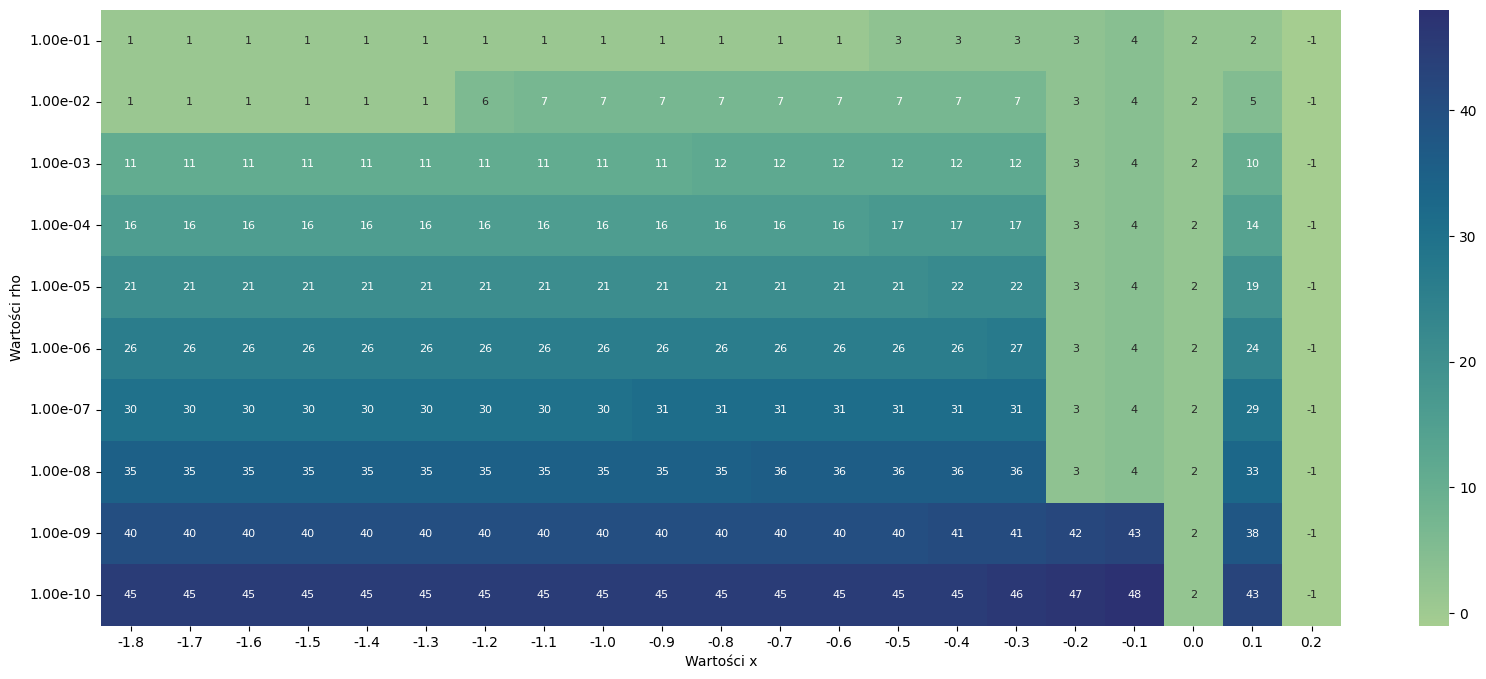
\includegraphics[width=\textwidth]{heatmap22.png}
  \end{minipage}
  \caption{Wykres liczby iteracji w zależności od \(\rho\) i \(x\)}
\end{figure}

\noindent
W tabli poniżej przedstawiona została druga najlepsza otrzymana wartość przybliżenia (Oraz liczba iteracji, \(\rho\) i początkowe x dla którego została otrzymana) dla danych wartości prametru \(\rho\) oraz kryterium stopu w zestaweniu z prawdziwą wartością pierwiastka.

\begin{table}[H]
    \centering
    \begin{tabular}{|l|l|}
    \hline
        Prawdziwa wartość pierwiastka & 0.0 \\ \hline
        Najlepsze przybliżenie & -1.1e-10 \\ \hline
        Liczba iteracji & 103 \\ \hline
        Wartość $\rho$ & 1.0e-10 \\ \hline
        Początek przedziału & -0.2 \\ \hline
        Koniec przedziału & 0.2 \\ \hline
    \end{tabular}
    \caption{Wartość drugiego najlepszego przybliżenia}
\end{table}

\subsubsection{Wartość bezwzględna różnicy dwóch ostatnich przybliżeń pierwiastka, \(\rho \in [10^{-11}, 10^{-20}]\), koniec przedziału ustalony na 0.2}

W tym przypadku już przybliżenie w każdej sytuacji jest dobre, i polepsza się wraz z zmniejszeniem wartości \(\rho\).

\begin{figure}[H]
  \centering
  \begin{minipage}[b]{0.9\textwidth}
    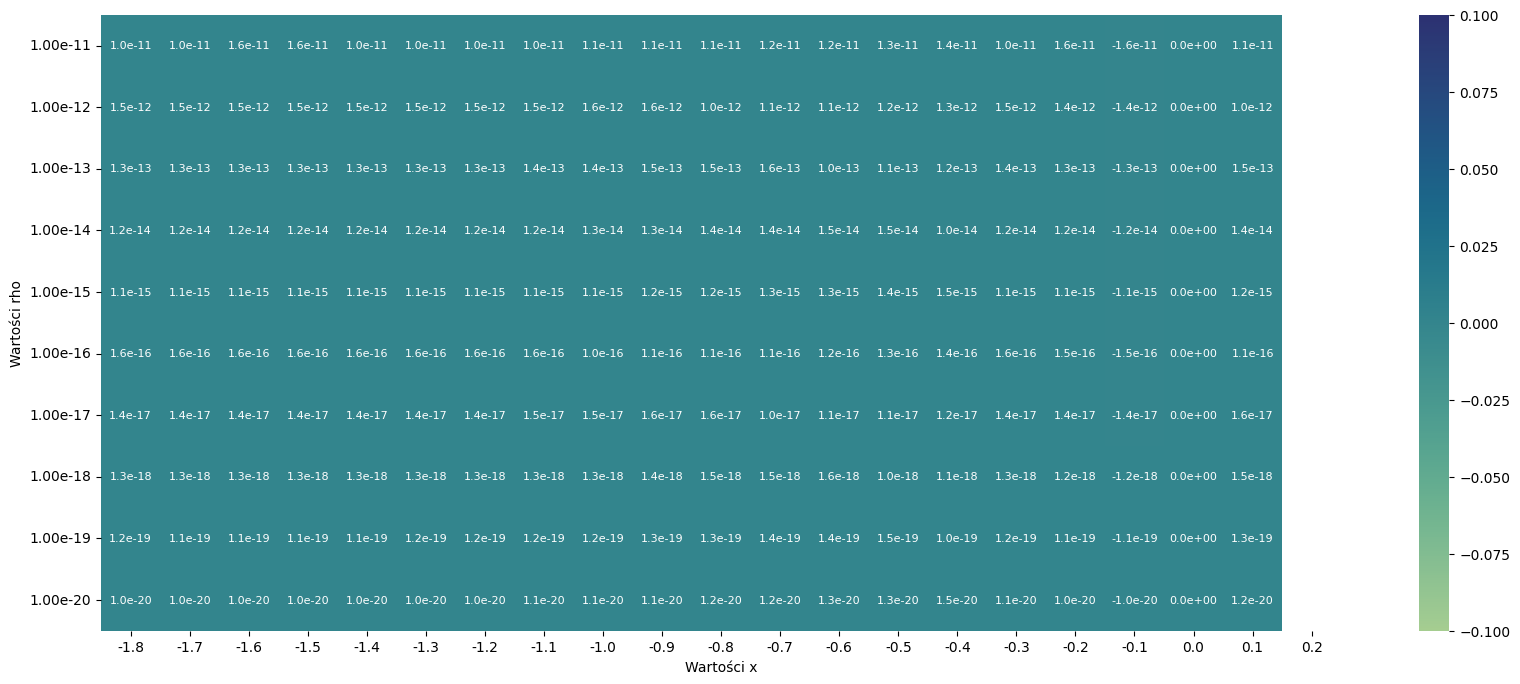
\includegraphics[width=\textwidth]{heatmap23.png}
  \end{minipage}
  \caption{Wykres wartości pierwiastka w zależności od \(\rho\) i \(x\)}
\end{figure}

\begin{figure}[H]
  \centering
  \begin{minipage}[b]{0.9\textwidth}
    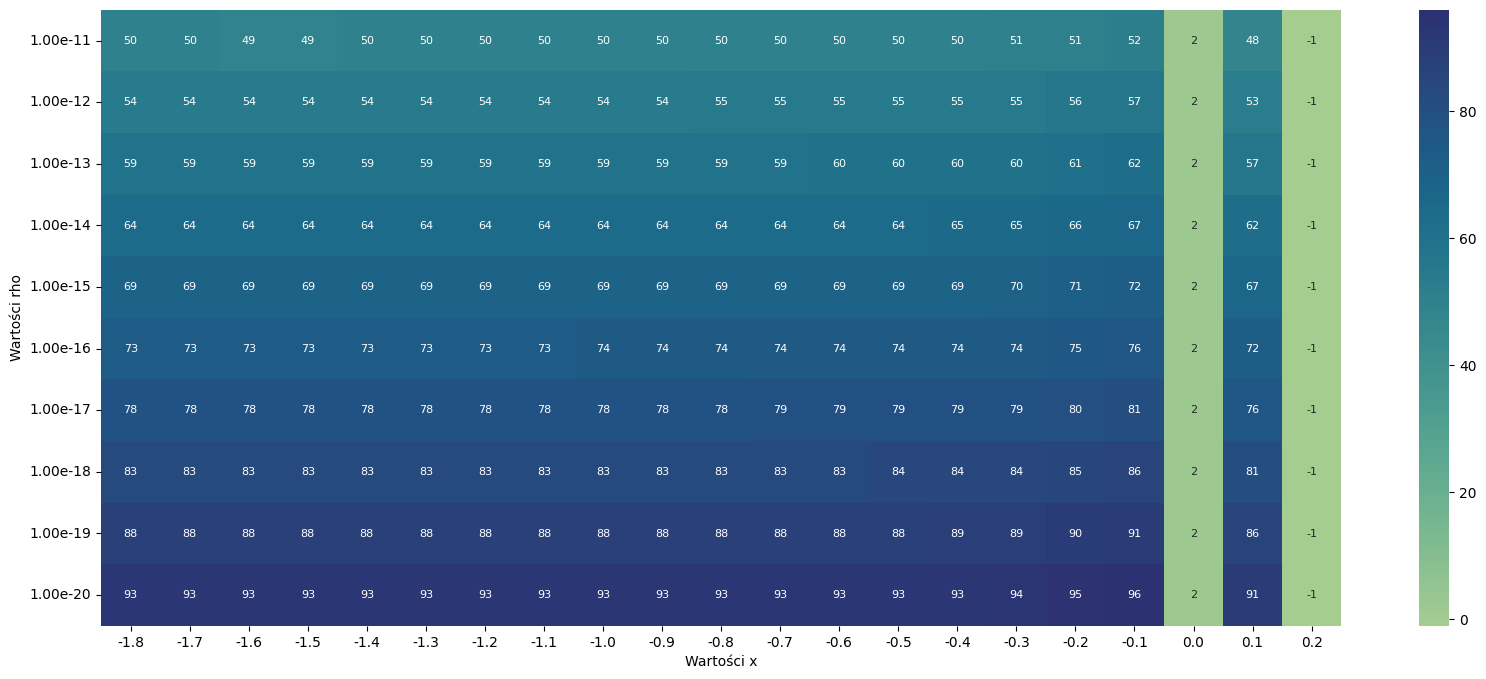
\includegraphics[width=\textwidth]{heatmap24.png}
  \end{minipage}
  \caption{Wykres liczby iteracji w zależności od \(\rho\) i \(x\)}
\end{figure}

\noindent
Z uwagi na to, że za każdym razem dla przedziału, który kończy lub zaczyna od 0.0 otrzymuję dokładną wartość pierwiastka. Pominąłęm ją w tym zestawieniu i w tabli poniżej przedstawiona została druga najlepsza otrzymana wartość przybliżenia (Oraz liczba iteracji, \(\rho\) i początkowe x dla którego została otrzymana) dla danych wartości prametru \(\rho\) oraz kryterium stopu w zestaweniu z prawdziwą wartością pierwiastka.


\begin{table}[H]
    \centering
    \begin{tabular}{|l|l|}
    \hline
        Prawdziwa wartość pierwiastka & 0.0 \\ \hline
        Najlepsze przybliżenie & -1.0e-20 \\ \hline
        Liczba iteracji & 95 \\ \hline
        Wartość $\rho$ & 1.0e-20 \\ \hline
        Początek przedziału & -0.2 \\ \hline
        Koniec przedziału & 0.2 \\ \hline
    \end{tabular}
\end{table}

\section{Porównanie efektywności obu algorytmów}

Na poniższych wykresach (25 i 26) wyraźnie widać, że metoda siecznych wykonuje znacznie więcej iteracji od metody newtona. Obie metody przy odpowiednio dobranym \(\rho\) dają akceptowalny wynik.

\begin{figure}[H]
  \centering
  \begin{minipage}[b]{\textwidth}
    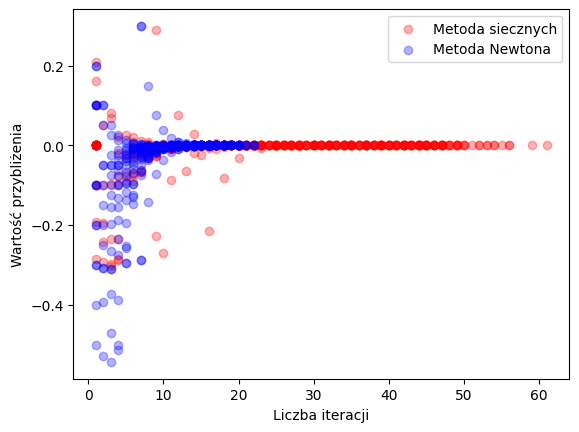
\includegraphics[width=\textwidth]{img25.png}
  \end{minipage}
  \caption{Porównanie metody Newtona i Siecznych dla kryterium wartości bezwzględnej}
\end{figure}

\begin{figure}[H]
  \centering
  \begin{minipage}[b]{\textwidth}
    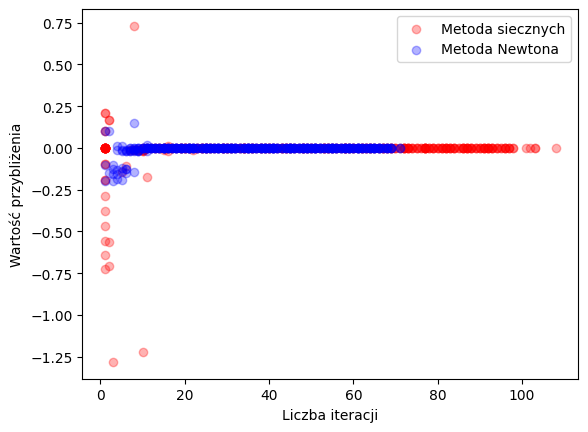
\includegraphics[width=\textwidth]{img26.png}
  \end{minipage}
  \caption{Porównanie metody Newtona i Siecznych dla kryterium wartości bezwzględnej różnicy dwóch ostatnich przybliżeń pierwiastka}
\end{figure}

\section{Najlepsze otrzymane przybliżenie}

Najlepsze przybliżenie otrzymałem przy wykorzystaniu metody siecznych, ustaleniu początku lub końca przedziału \(x = 0.0\) i dowolnej wartości \(\rho\). Powodem tego jest, to że funkcja f dla wartości 0 również zwraca 0.

\section{Wnioski}

\begin{itemize}
    \item Metoda Newtona wykonuje znacznie mniej iteracji i często zwraca lepsze przybliżenie
    \item Metoda siecznych nie wymaga znania pochodnej funkcji, co może być dużą zaletą
\end{itemize}

\end{document}
